% !TeX document-id = {3c9fb181-ef8d-46f4-a369-f483876e4c37}
% !TeX TXS-program:compile = txs:///pdflatex/[--shell-escape]

\documentclass[fleqn,11pt,aspectratio=169]{beamer}
\usepackage{tubslogo}
\usepackage{amsmath}
\usepackage{amsfonts}
\usepackage{amssymb}
\usepackage{graphicx}
\usepackage{geometry}
\usepackage{tikz}
\usepackage{amsthm}
\usepackage{float}
\usepackage{cleveref}
\usepackage{acronym}

\usepackage{fancyvrb}
\usepackage{fvextra}
\usepackage[normalem]{ulem}
\usepackage{enumerate}

\usepackage[overload]{textcase}
\usepackage{minitoc}        
%\usepackage{etoc}        
\usepackage{printlen}
\usepackage{url}  
\usepackage{tabularx}  
\usepackage{soul}
\usepackage{siunitx}
\usepackage{eqparbox}
\sisetup{
	per-mode=symbol,
}
\usepackage[utf8]{inputenc}
\usepackage[
	backend=biber,
	style=numeric,
]{biblatex}

\usepackage[rgb,dvipsnames]{xcolor}

\selectcolormodel{natural}
\usepackage{ninecolors}
\selectcolormodel{rgb}
\usepackage{tabularray}
\usepackage{minted}
\usemintedstyle{emacs,tabsize=2,linenos,xleftmargin=10pt,highlightcolor=cyan}

\usepackage[export]{adjustbox}% http://ctan.org/pkg/adjustbox

\usepackage[append]{beamersubframe}
\usepackage[american]{babel}
\usepackage{graphicx}
\setbeamerfont{normal text}{size=12pt}

\date{April 23, 2026}
\usetheme[%
  %nexus,%        Nexus Fonts benutzen
  %lnum,%         Versalziffern verwenden
  %cmyk,%<rgbprint>,          Auswahl des Farbmodells
  blue,%<orange/green/violet> Auswahl des Sekundärfarbklangs
  dark,%<light,medium>        Auswahl der Helligkeit
  %colorhead,%    Farbig hinterlegte Kopfleiste
  %colorfoot,%    Farbig hinterlegt Fußleiste auf Titelseite
  colorblocks,%   Blöcke Farbig hinterlegen
  %nopagenum,%    Keine Seitennumer in Fußzeile
  %nodate,%       Kein Datum in Fußleiste
  tocinheader,%   Inhaltsverzeichnis in Kopfleiste
  %tinytocinheader,% kleines Kopfleisten-Inhaltsverzeichnis
  %widetoc,%      breites Kopfleisten-Inhaltsverzeichnis
  %narrowtoc,%    schmales Kopfleisten-Inhaltsverzeichnis
  %nosubsectionsinheader,%  Keine subsections im Kopfleisten-Inhaltsverzeichnis
  %nologoinfoot,% Kein Logo im Fußbereich darstellen
  ]{tubs}
% Titelseite
%\title{towards TPU: A Survey into Accelerators for Cloud AI}
\title{Algorithm Engineering 2026: Sheet 02}
\author{Rouven Kniep}

%titlepage font and background
\setbeamercolor{titlebarfirst}{parent=titlepage, bg=titlepage.bg!0}

% Edit the TUBS template to move the tubslogo into place for the title
\let\tubslogoAbsOld\tubslogoAbs
\renewcommand{\tubslogoAbs}[1]{\raisebox{-2.3mm}{\tubslogoAbsOld{#1}}}

% Quoteblock 
\newcommand{\quotebox}[1]{\begin{center}\fcolorbox{white}{blue!15!gray!15}{\begin{minipage}{0.9\linewidth}\vspace{10pt}\center\begin{minipage}{0.8\linewidth}{\space\Huge``}{#1}{\hspace{1.5em}\break\null\Huge\hfill''}\end{minipage}\smallbreak\end{minipage}}\end{center}}



\begin{document}

\part{main}
\begin{frame}[plain]
	\titlepage
\end{frame}	

\section{Ex1a}

\begin{frame}{Ex1: Setting}
	\begin{columns}[T]
		\column{0.4\textwidth}
		Data Structures
		\begin{itemize}
			\item Adjacency List
			\begin{itemize}
				\item Array of Structs
				\item Struct of Arrays
			\end{itemize}
			\item Compressed Sparse Row			
			\begin{itemize}
				\item vector
				\item sorted vector
				\item \texttt{std::unordered\_map}\\
					 $\implies$ hash as key to array of linked lists
			\end{itemize}
		\end{itemize}
		
		\column{0.55\textwidth}
		Graphs
		\begin{tblr}{colspec={c|c|c|X}, width=\columnwidth}
			G & Vertices & Density & Notes \\
			\hline
			1 &  1000 & medium & Erd\H{o}s-Renyi \\
			\hline
			2 &  200 & very dense & Erd\H{o}s-Renyi \\
			\hline
			3 &  100000 & sparse & \\
			\hline
			\SetCell[r=2]{} 4 & 100000 & sparser & \SetCell[r=2]{}{usually sparse, \newline high-degree}\\
			& 100 & dense & \\
		\end{tblr}
		
	\end{columns}
\end{frame}

\begin{frame}{1a: Data}
	\begin{center}
		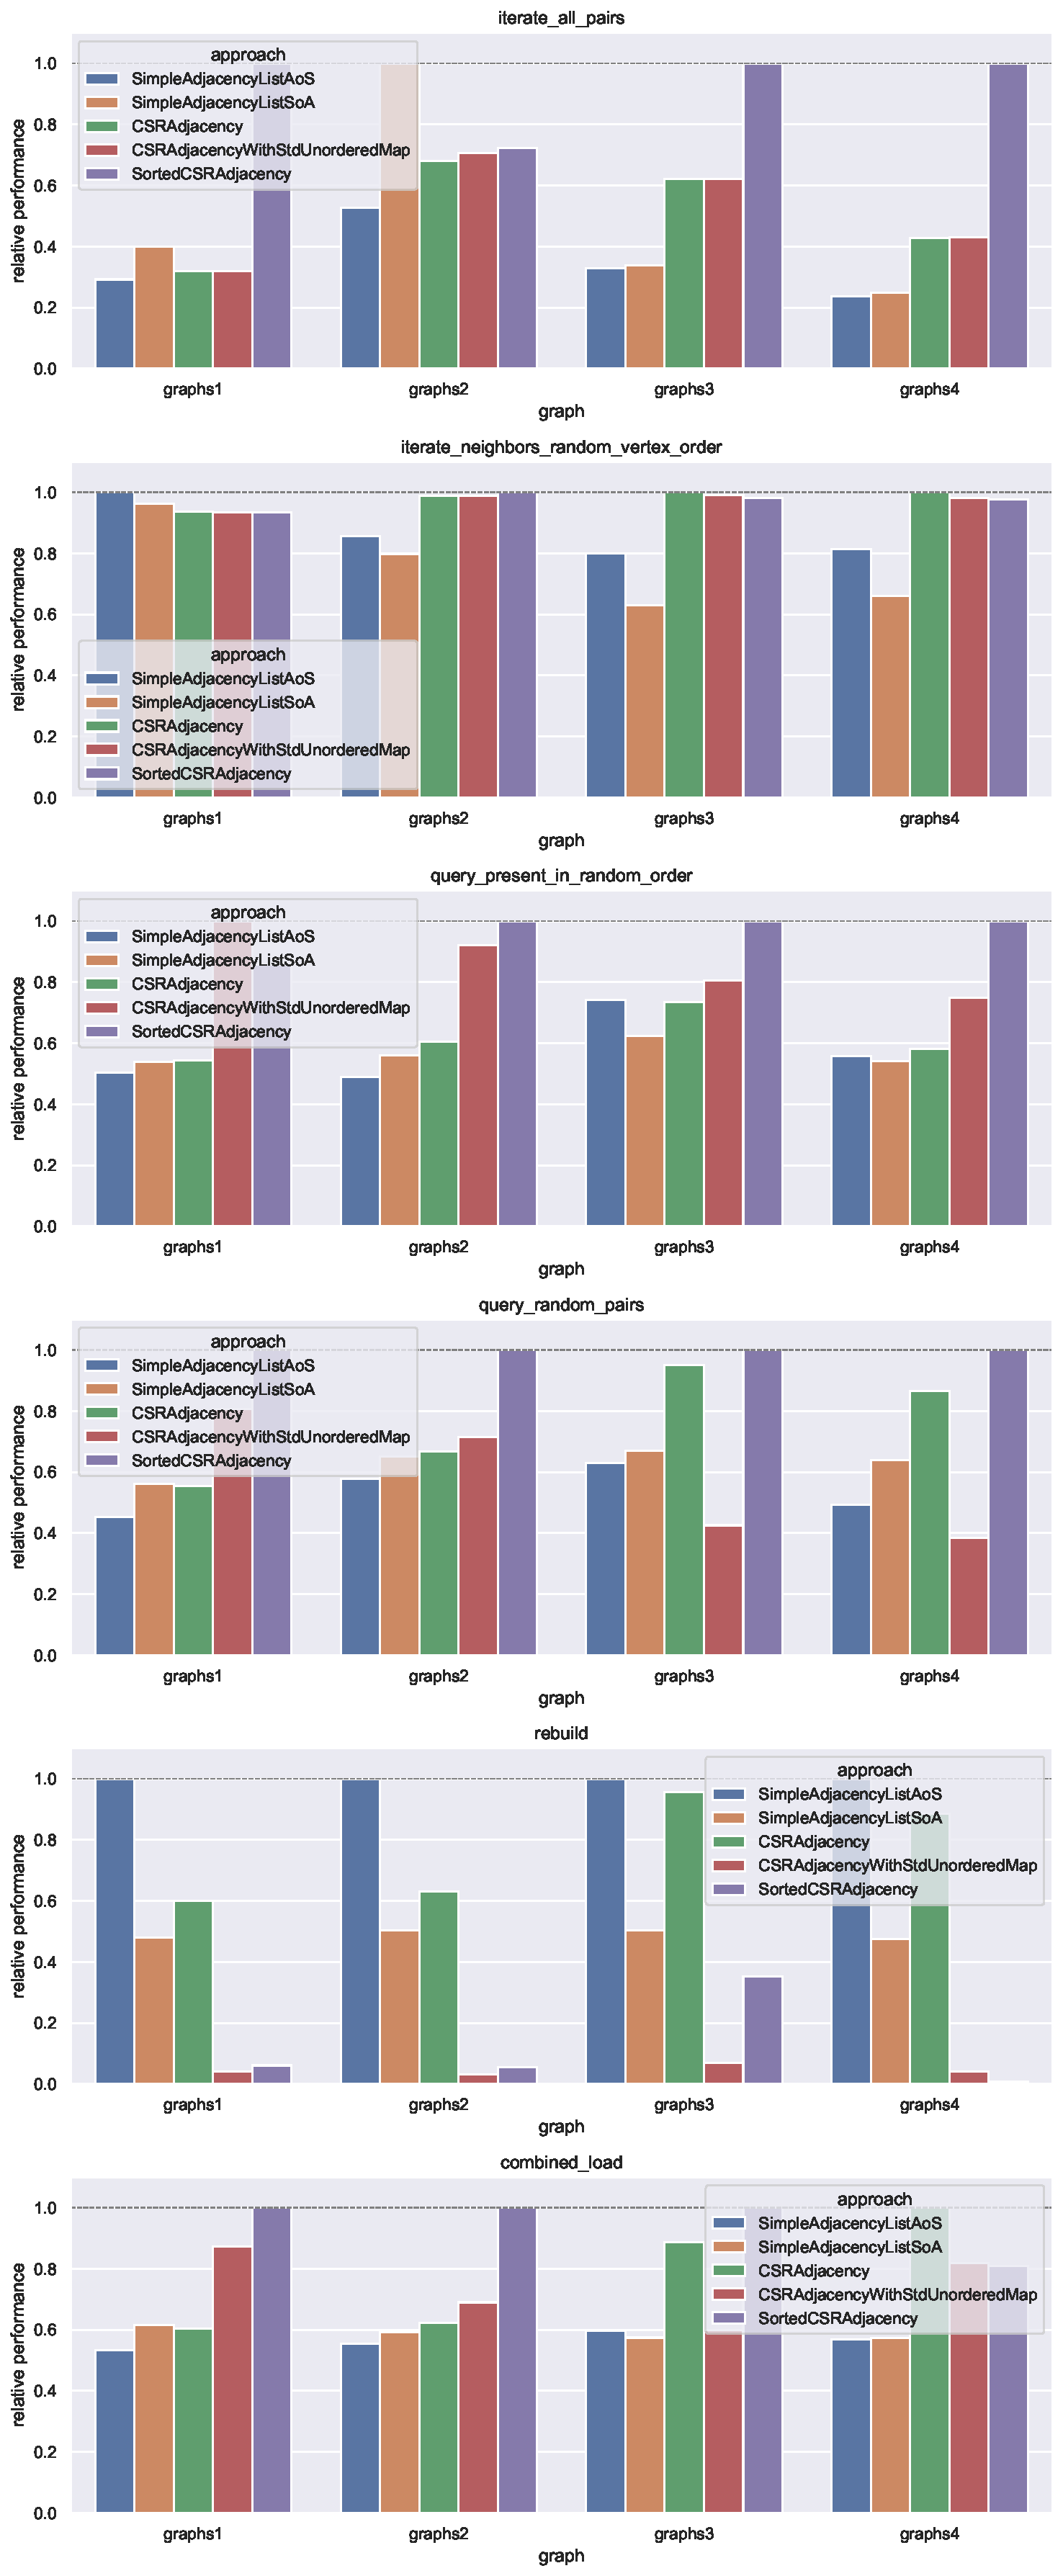
\includegraphics[keepaspectratio, clip, trim={0 19.9in 0 0}, width=0.95\textwidth]{../../homework/HW02/benchmark-results.pdf}
		
		\begin{tblr}{colspec={l *{4}{X[c]}}, width=\linewidth}
			\hspace{0.05\linewidth}& few vertices, medium dense & very few vertices, very dense & many vertices, sparse & many vertices, most very sparse \\ 
		\end{tblr}
	\end{center}
\end{frame}

	
\begin{frame}{Nested Vector memory layout...}
	\begin{tblr}{colspec={r| *{8}{X[c]}}, width=\linewidth}
		addr & \SetCell[c=8]{} line 64 byte &&&&&&&\\
		\hline
		\texttt{0x00}	&&& \SetCell[c=3]{Gray} global header &&&&&\\
		\hline
		\hline
		\texttt{0x180} & \SetCell{Yellow} elem &\SetCell{Yellow} elem &\SetCell{Yellow} elem &\SetCell{Yellow} elem &\SetCell{Yellow} elem &\SetCell{Yellow} elem & & \\
		\hline
		\hline
		\texttt{0x10B0}	& \SetCell[c=3]{Yellow} Yellow header &&& \SetCell[c=3]{Cyan} Cyan Header &&& \SetCell[c=2]{Salmon} Salmon header &\\
		\texttt{0x1100}	& \SetCell[c=1]{Salmon} Salmon &&&&&&&\\
		\hline
		\hline
		\texttt{0x3780} & \SetCell{Salmon} elem &\SetCell{Salmon} elem &\SetCell{Salmon} elem &\SetCell{Salmon} elem &&&& \\
		\hline
		\hline
		\texttt{0xF400} & \SetCell{Cyan} elem &\SetCell{Cyan} elem &\SetCell{Cyan} elem &\SetCell{Cyan} elem &\SetCell{Cyan} elem &\SetCell{Cyan} elem &\SetCell{Cyan} elem &\SetCell{Cyan} elem \\
		\texttt{0xF440} & \SetCell{Cyan} elem &\SetCell{Cyan} elem &&&&&& \\
	\end{tblr}
\end{frame}


\begin{frame}{Compressed Sparse Row (CSR) memory layout...}
	\begin{tblr}{colspec={r| *{8}{X[c]}}, width=\linewidth}
		addr & \SetCell[c=8]{} line 64 byte &&&&&&&\\
		\hline
		\texttt{0x00}	& \SetCell[c=3]{Gray} main header &&&& \SetCell[c=3]{Gray} endmarker header &&&\\
		\hline
		\hline
		\texttt{0x10B0} & \SetCell{Yellow} elem &\SetCell{Yellow} elem &\SetCell{Yellow} elem &\SetCell{Yellow} elem &\SetCell{Yellow} elem &\SetCell{Yellow} elem & \SetCell{Cyan} elem &\SetCell{Cyan} elem \\
		\texttt{0x1100} & \SetCell{Cyan} elem & \SetCell{Cyan} elem & \SetCell{Cyan} elem &\SetCell{Cyan} elem &\SetCell{Cyan} elem &\SetCell{Cyan} elem & \SetCell{Cyan} elem &\SetCell{Cyan} elem \\
		\texttt{0x1140} & \SetCell{Salmon} elem &\SetCell{Salmon} elem &\SetCell{Salmon} elem &\SetCell{Salmon} elem &&&& \\
		\hline
		\hline
		\texttt{0xF400} & \SetCell{Yellow} end & \SetCell{Cyan} end  & \SetCell{Salmon} end &&&&&\\
	\end{tblr}
	
	\vspace{10pt}	
	
	\centering \large $\implies$ much better linearity and efficiency for low degrees!
\end{frame}

\begin{frame}[fragile]{CSR vs sorted CSR \texttt{for\_each} performance}
\centering same code, relevant section:

\begin{minted}[highlightlines={}]{c++}
for (Index i = start; i < end; ++i) {
	Index partner = m_partners[i]; 
	if (partner < u) { continue; }
	Index pair_index = m_pair_indices[i];
	if constexpr(result_is_boolean) {
		if (!static_cast<bool>(
		std::invoke(std::forward<Callable>(func),
		u, partner, pair_index))
		) { return; }
	} else {
		std::invoke(std::forward<Callable>(func), u, partner, pair_index);
	}
}
\end{minted}
\end{frame}

\begin{frame}[fragile,noframenumbering]{CSR vs sorted CSR \texttt{for\_each} performance}
\centering \texttt{m\_pair\_indices}: data only, no program flow impact
	
\begin{minted}[highlightlines={4,8,11}]{c++}
for (Index i = start; i < end; ++i) {
	Index partner = m_partners[i]; 
	if (partner < u) { continue; }
	Index pair_index = m_pair_indices[i];      // load from memory..
	if constexpr(result_is_boolean) {
		if (!static_cast<bool>(
		std::invoke(std::forward<Callable>(func),  
		u, partner, pair_index))    // and feed into the invoked function
		) { return; }
	} else {
		std::invoke(std::forward<Callable>(func), u, partner, pair_index);
	}
}
\end{minted}
\end{frame}

\begin{frame}[fragile,noframenumbering]{CSR vs sorted CSR \texttt{for\_each} performance}
\centering \texttt{m\_partners}: unsorted case

\begin{minted}[highlightlines={2,3}]{c++}
for (Index i = start; i < end; ++i) {
	Index partner = m_partners[i];   // load from memory, data unsorted
	if (partner < u) { continue; }   // branch -> cosly mispredictions
	Index pair_index = m_pair_indices[i];      
	if constexpr(result_is_boolean) {
		if (!static_cast<bool>(
		std::invoke(std::forward<Callable>(func),  
		u, partner, pair_index))
		) { return; }
	} else {
		std::invoke(std::forward<Callable>(func), u, partner, pair_index);
	}
}
\end{minted}
\end{frame}

\begin{frame}[fragile,noframenumbering]{CSR vs sorted CSR \texttt{for\_each} performance}
\centering \texttt{m\_partners}: sorted case
	
\begin{minted}[highlightlines={2,3}]{c++}
for (Index i = start; i < end; ++i) {
	Index partner = m_partners[i];   // load from memory, data sorted
	if (partner < u) { continue; }   // branch -> less mispredictions
	Index pair_index = m_pair_indices[i];      
	if constexpr(result_is_boolean) {
		if (!static_cast<bool>(
		std::invoke(std::forward<Callable>(func),  
		u, partner, pair_index))
		) { return; }
	} else {
		std::invoke(std::forward<Callable>(func), u, partner, pair_index);
	}
}
\end{minted}
\end{frame}

\section{Ex1b}

\begin{frame}{Cache Lines}
	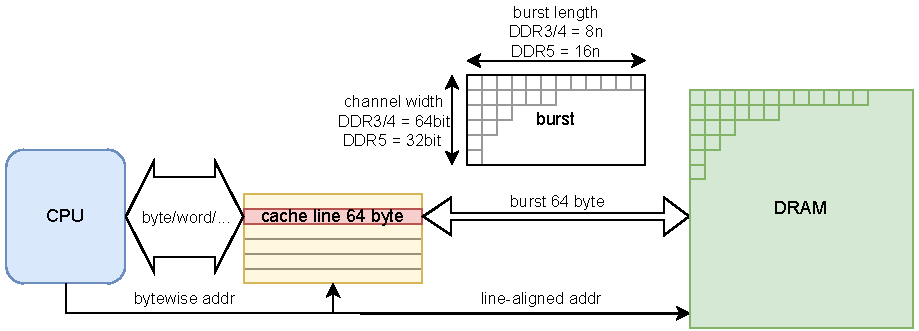
\includegraphics[width=\linewidth, keepaspectratio]{CPU_memory_cachelines.pdf}
\end{frame}

\begin{frame}{Eytzinger-Layout}
	from: \href{https://algorithmica.org/en/eytzinger}{https://algorithmica.org/en/eytzinger}
	\begin{columns}
		\column{0.5\textwidth}
		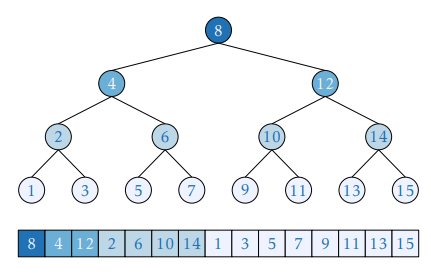
\includegraphics[keepaspectratio, width=\columnwidth]{eytzinger.png}
		
		\column{0.45\textwidth}
		\begin{itemize}
			\item smaller child: $2k$
			\item bigger child: $2k+1$
			\item children in $d$ steps: \\in $[2^d*k, 2^{d+1}*k)$
		\end{itemize}
	\end{columns}
	\begin{center}
	\end{center}
\end{frame}

\begin{frame}{Eytzinger in memory}
\begin{tblr}{colspec={|X[c]|X[c]|X[c]|X[c]|X[c]|X[c]|X[c]|X[c]|}, row{3}=Yellow, row{4,5}=Green, width=\linewidth}
	\SetCell[c=8]{} line 64 byte, elements 8 byte &&&&&&&\\
	empty & \SetCell{Apricot} 1 (root) & \SetCell{Cerulean} 2 & \SetCell{Cerulean} 3 & \SetCell{WildStrawberry} 4 & \SetCell{WildStrawberry} 5 & \SetCell{WildStrawberry} 6 & \SetCell{WildStrawberry} 7 \\
	8 & 9 & 10 & 11 & 12 & 13 & 14 & 15 \\
	16 & 17 & 18 & 19 & 20 & 21 & 22 & 23 \\
	24 & 25 & 26 & 27 & 28 & 29 & 30 & 31 \\
\end{tblr}
\begin{center}
	\begin{itemize}
		\item can prefetch an aligned line *without cost* $d$ steps in advance, with \\
		
		$d=log_2(\frac{|l|}{|e|})=log_2(\frac{\qty{64}{\byte}}{\qty{64}{\bit}})=3$ 
		
		\item $\implies$ more efficient for small data types
		\item requires software prefetching: \\\texttt{\_\_builtin\_prefetch(base + k * 64/sizeof(node\_type\_t);}
		\item potentially even prefetching multiple lines
		\item requires alignment: \texttt{alignas(64) node\_type\_t base[n+1]}
	\end{itemize}		
\end{center}
\end{frame}

\begin{frame}{Eytzinger-Layout: Caveats}
	graphic from: \href{https://algorithmica.org/en/eytzinger}{https://algorithmica.org/en/eytzinger}
	\begin{columns}
		\column{0.5\textwidth}
		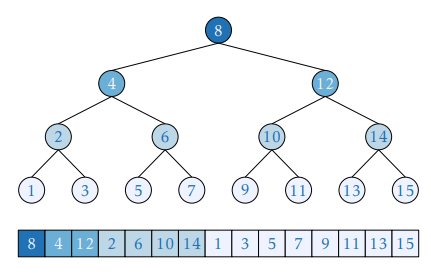
\includegraphics[keepaspectratio, width=\columnwidth]{eytzinger.png}
		
		\column{0.45\textwidth}
		\begin{itemize}
			\item performance gain up to $d = 3\times$ by pipelining away memory latency
			\item but low memory utilization: only $\frac{|e|}{|l|} = \frac{\qty{64}{\bit}}{\qty{64}{\byte}} = \frac{1}{8}$ bytes actually used
			\item $\implies$ bad in memory-constrained environments \\
				(which is basically anywhere) 
		\end{itemize}
	\end{columns}
	\begin{center}
	\end{center}
\end{frame}

\begin{frame}{B+-Trees ("Block"-Trees? b+1-ary Trees?)}
	\begin{center}
		note: this implementation is used in data base indices
	
		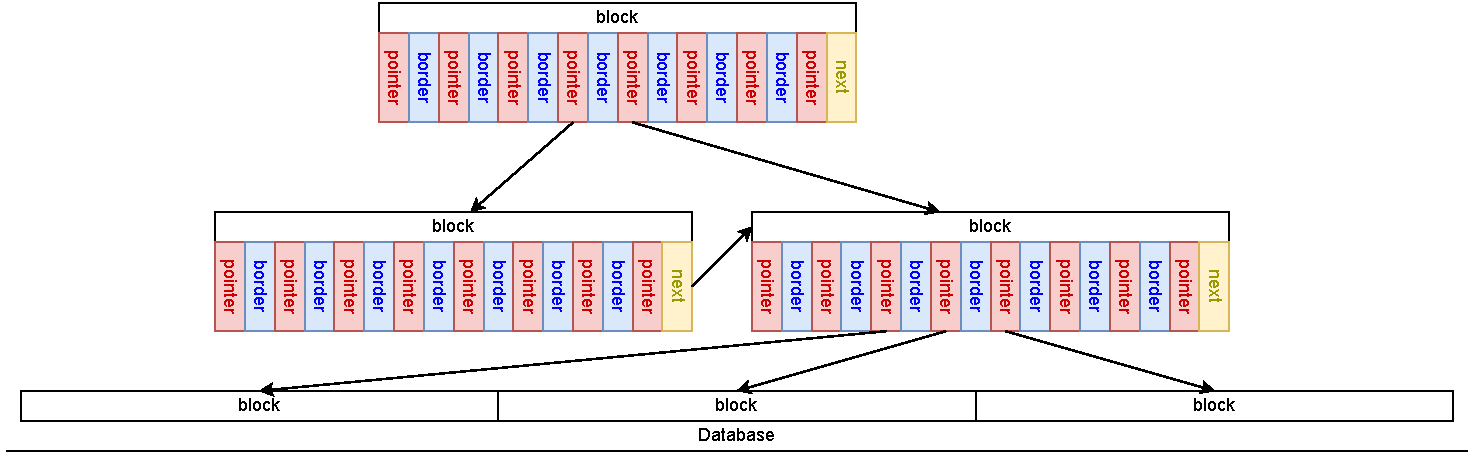
\includegraphics[keepaspectratio, width=\textwidth, page=1]{B+Tree.pdf}
	\end{center}
\end{frame}

\begin{frame}{implicit B-Trees}
	\begin{columns}
		\column{0.5\textwidth}
		\includegraphics[keepaspectratio, width=\columnwidth, page=2]{B+Tree.pdf}
		
		\column{0.4\textwidth}
		\begin{itemize}
			\item $b = \frac{|e|}{|l|} = 8$ elements per node
			\item $b+1$ children ("b+1-ary tree")
			\item when linearized: children of $k$ in $[(b+1)*k+1, (b+1)*k+b+1]$ \\
			\item shallow tree: depth $log_{b+1}(n)$
			\item memory-bandwidth friendlier
			\item but needs more compute
		\end{itemize}
	\end{columns}
\end{frame}

\begin{frame}[fragile]{\texttt{ImplicitBTreeCSRAdjacency::p\_get\_pair\_index} main loop}
\begin{minted}[]{c++}
__m256i block1_vec = _mm256_loadu_si256((const __m256i*)(&b[k*BLOCK_SIZE]));
block1_vec = _mm256_xor_si256(block1_vec, range_shift);
__m256i block2_vec = _mm256_loadu_si256((const __m256i*)(&b[k*BLOCK_SIZE+4]));
block2_vec = _mm256_xor_si256(block2_vec, range_shift);
__m256i mask1 = _mm256_cmpgt_epi64(search_vec, block1_vec);
__m256i mask2 = _mm256_cmpgt_epi64(search_vec, block2_vec);
unsigned m1 = _mm256_movemask_pd(_mm256_castsi256_pd(mask1));
unsigned m2 = _mm256_movemask_pd(_mm256_castsi256_pd(mask2));
unsigned mask = ~(m1 | (m2 << 4));
Index i = std::countr_zero(mask);
if(i < BLOCK_SIZE) { res = k * BLOCK_SIZE + i; }
k = go(k, i);
\end{minted}
\end{frame}

\section{Ex1c}
\begin{frame}{Performance: \texttt{iterate\_all\_pairs}}
	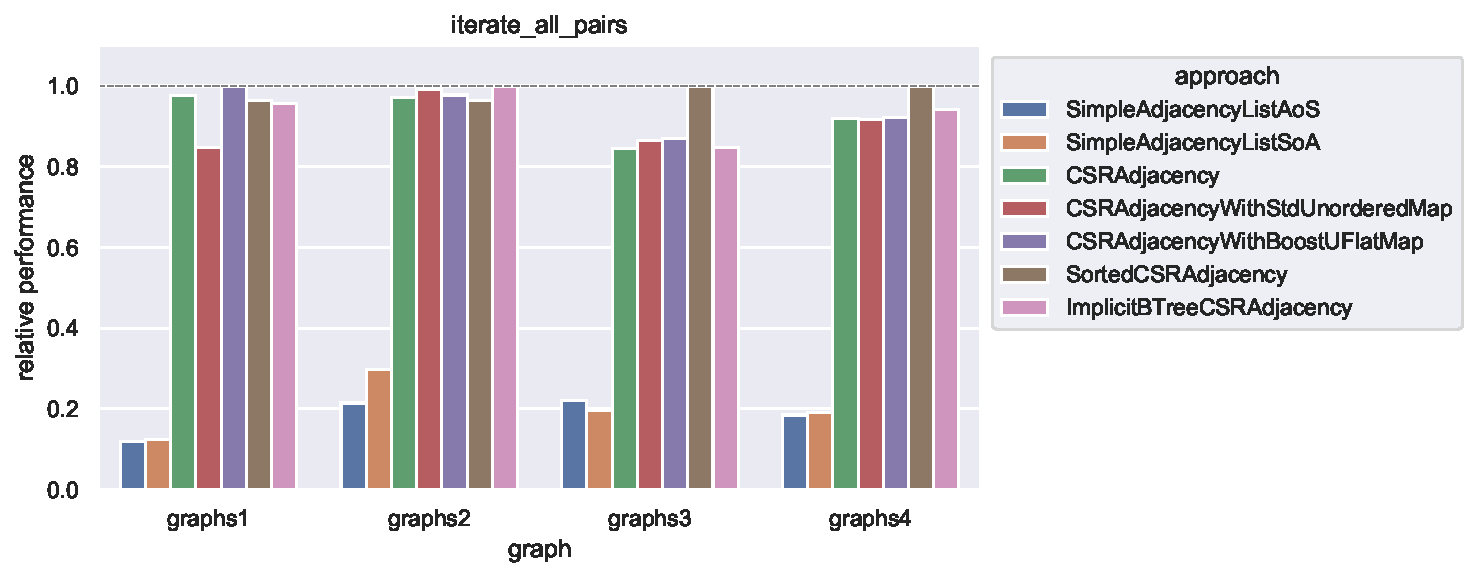
\includegraphics[width=\linewidth, keepaspectratio]{benchmark_iterate_all_pairs.pdf}
\end{frame}
\begin{frame}{Performance: \texttt{iterate\_neighbors\_random\_vertex\_order}}
	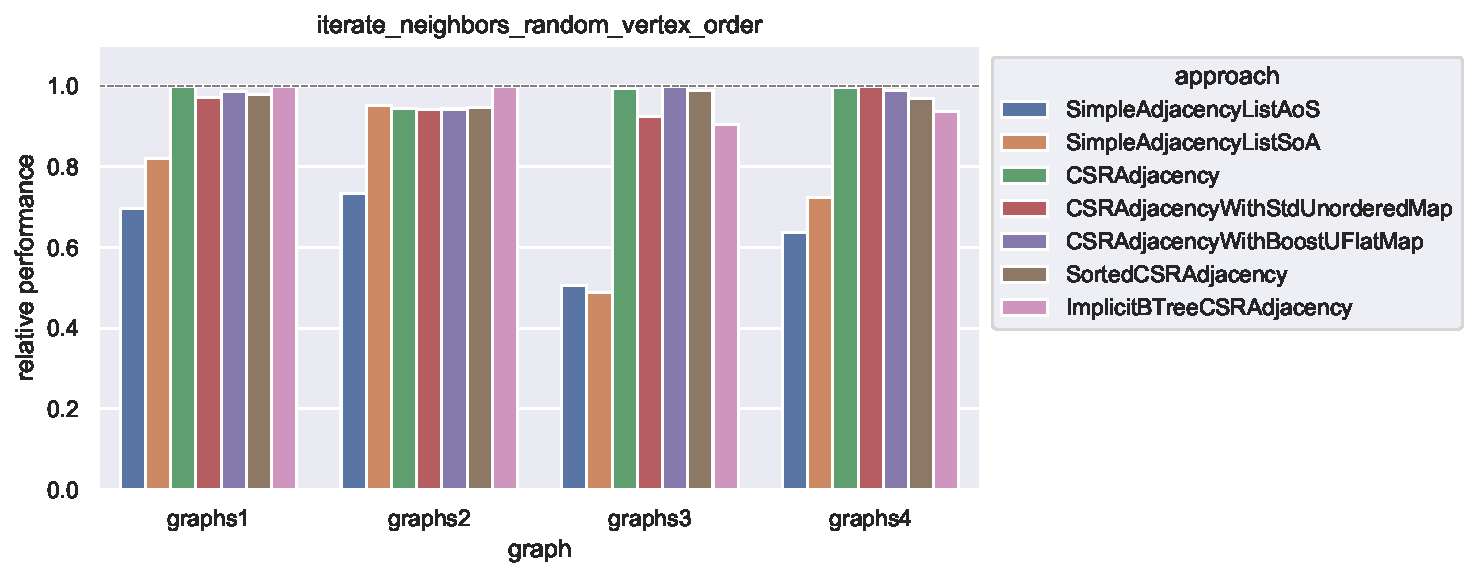
\includegraphics[width=\linewidth, keepaspectratio]{benchmark_iterate_neighbors_random_vertex_order.pdf}
\end{frame}
\begin{frame}{Performance: \texttt{query\_present\_in\_random\_order}}
	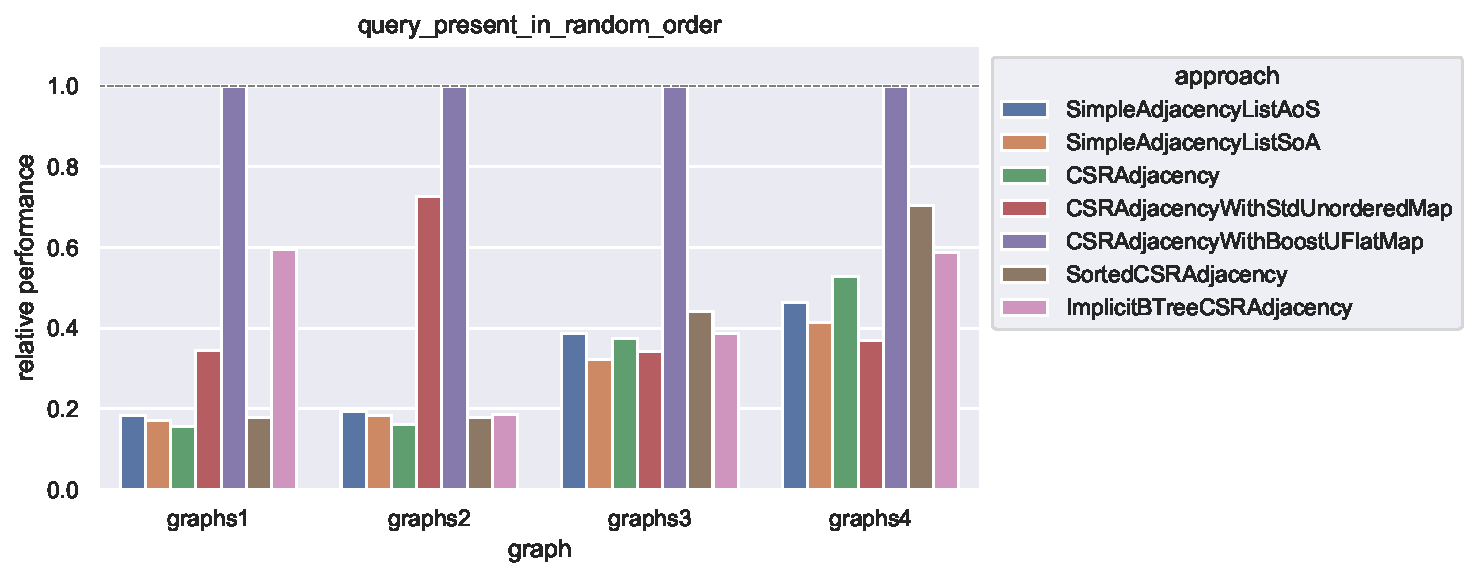
\includegraphics[width=\linewidth, keepaspectratio]{benchmark_query_present_in_random_order.pdf}
\end{frame}
\begin{frame}{Performance: \texttt{query\_random\_pairs}}
	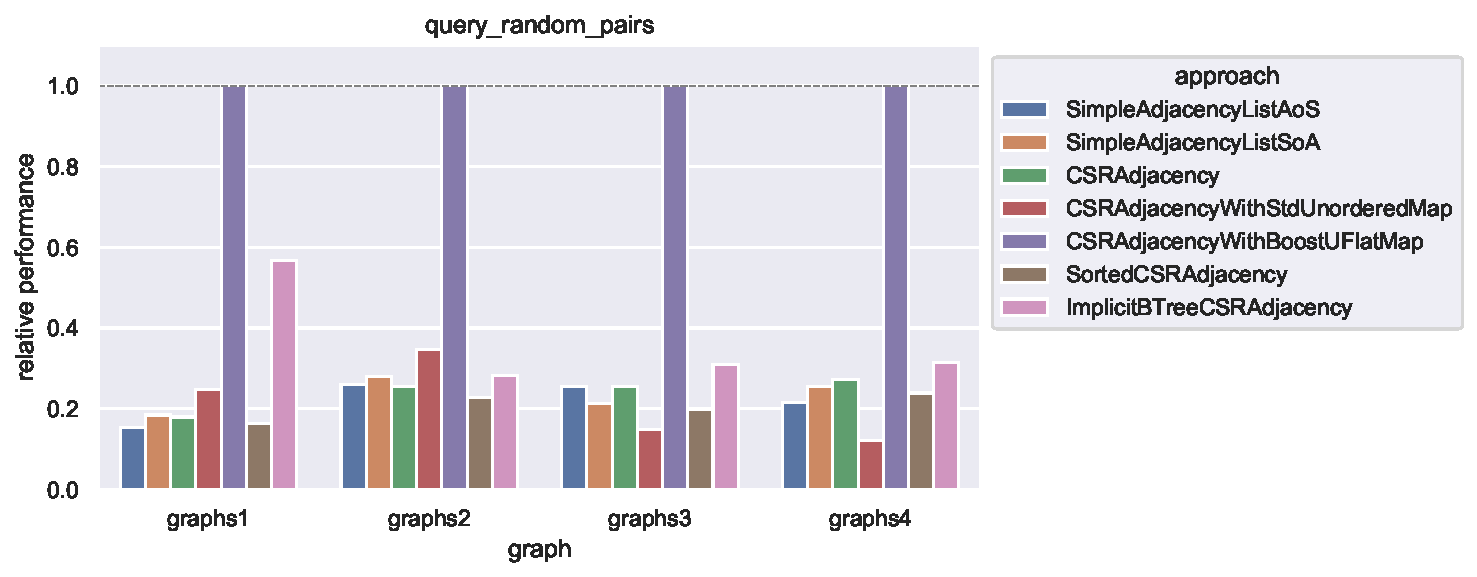
\includegraphics[width=\linewidth, keepaspectratio]{benchmark_query_random_pairs.pdf}
\end{frame}
\begin{frame}{Performance: \texttt{rebuild}}
	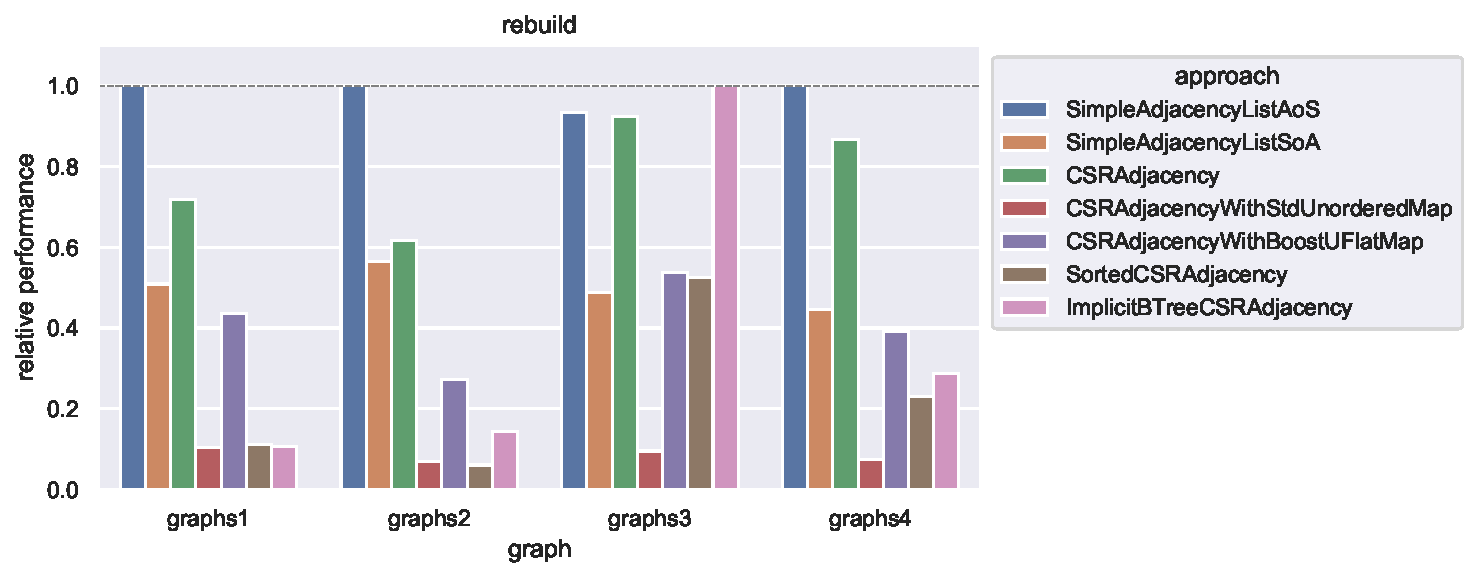
\includegraphics[width=\linewidth, keepaspectratio]{benchmark_rebuild.pdf}
\end{frame}
\begin{frame}{Performance: \texttt{combined\_load}}
	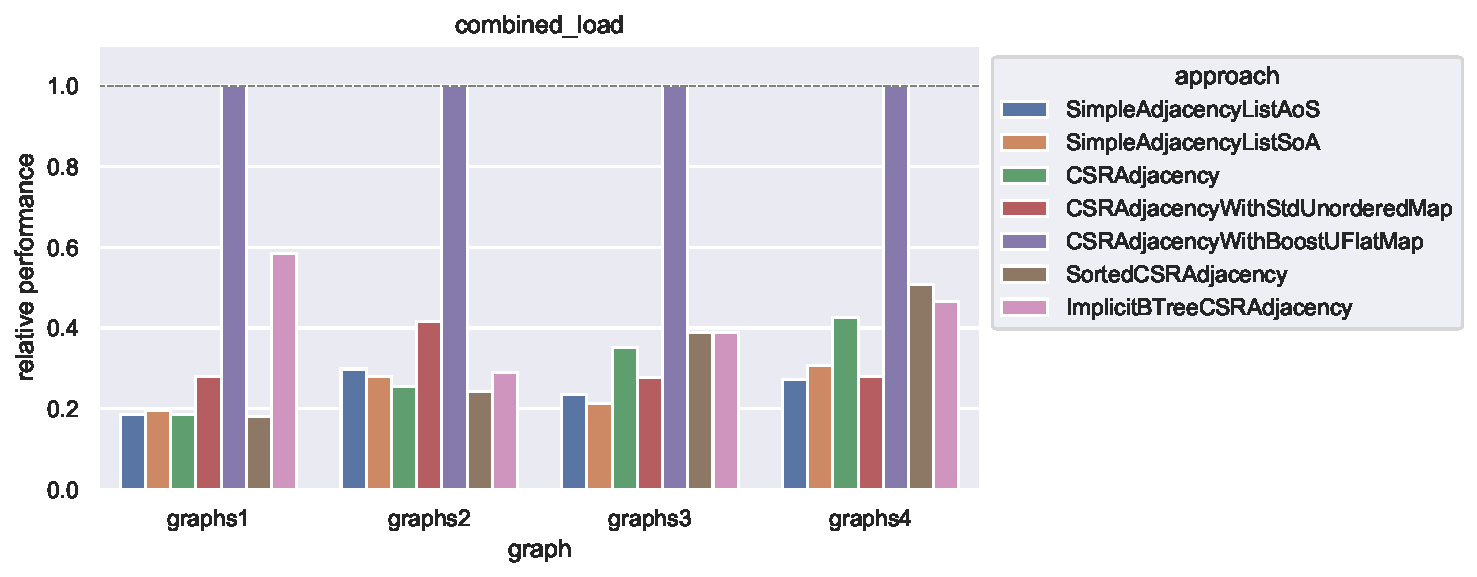
\includegraphics[width=\linewidth, keepaspectratio]{benchmark_combined_load.pdf}
\end{frame}


\section{Ex2}

\begin{frame}{failed Idea 1: Divide+Conquer}
	\begin{columns}
		\column{0.4\textwidth}
		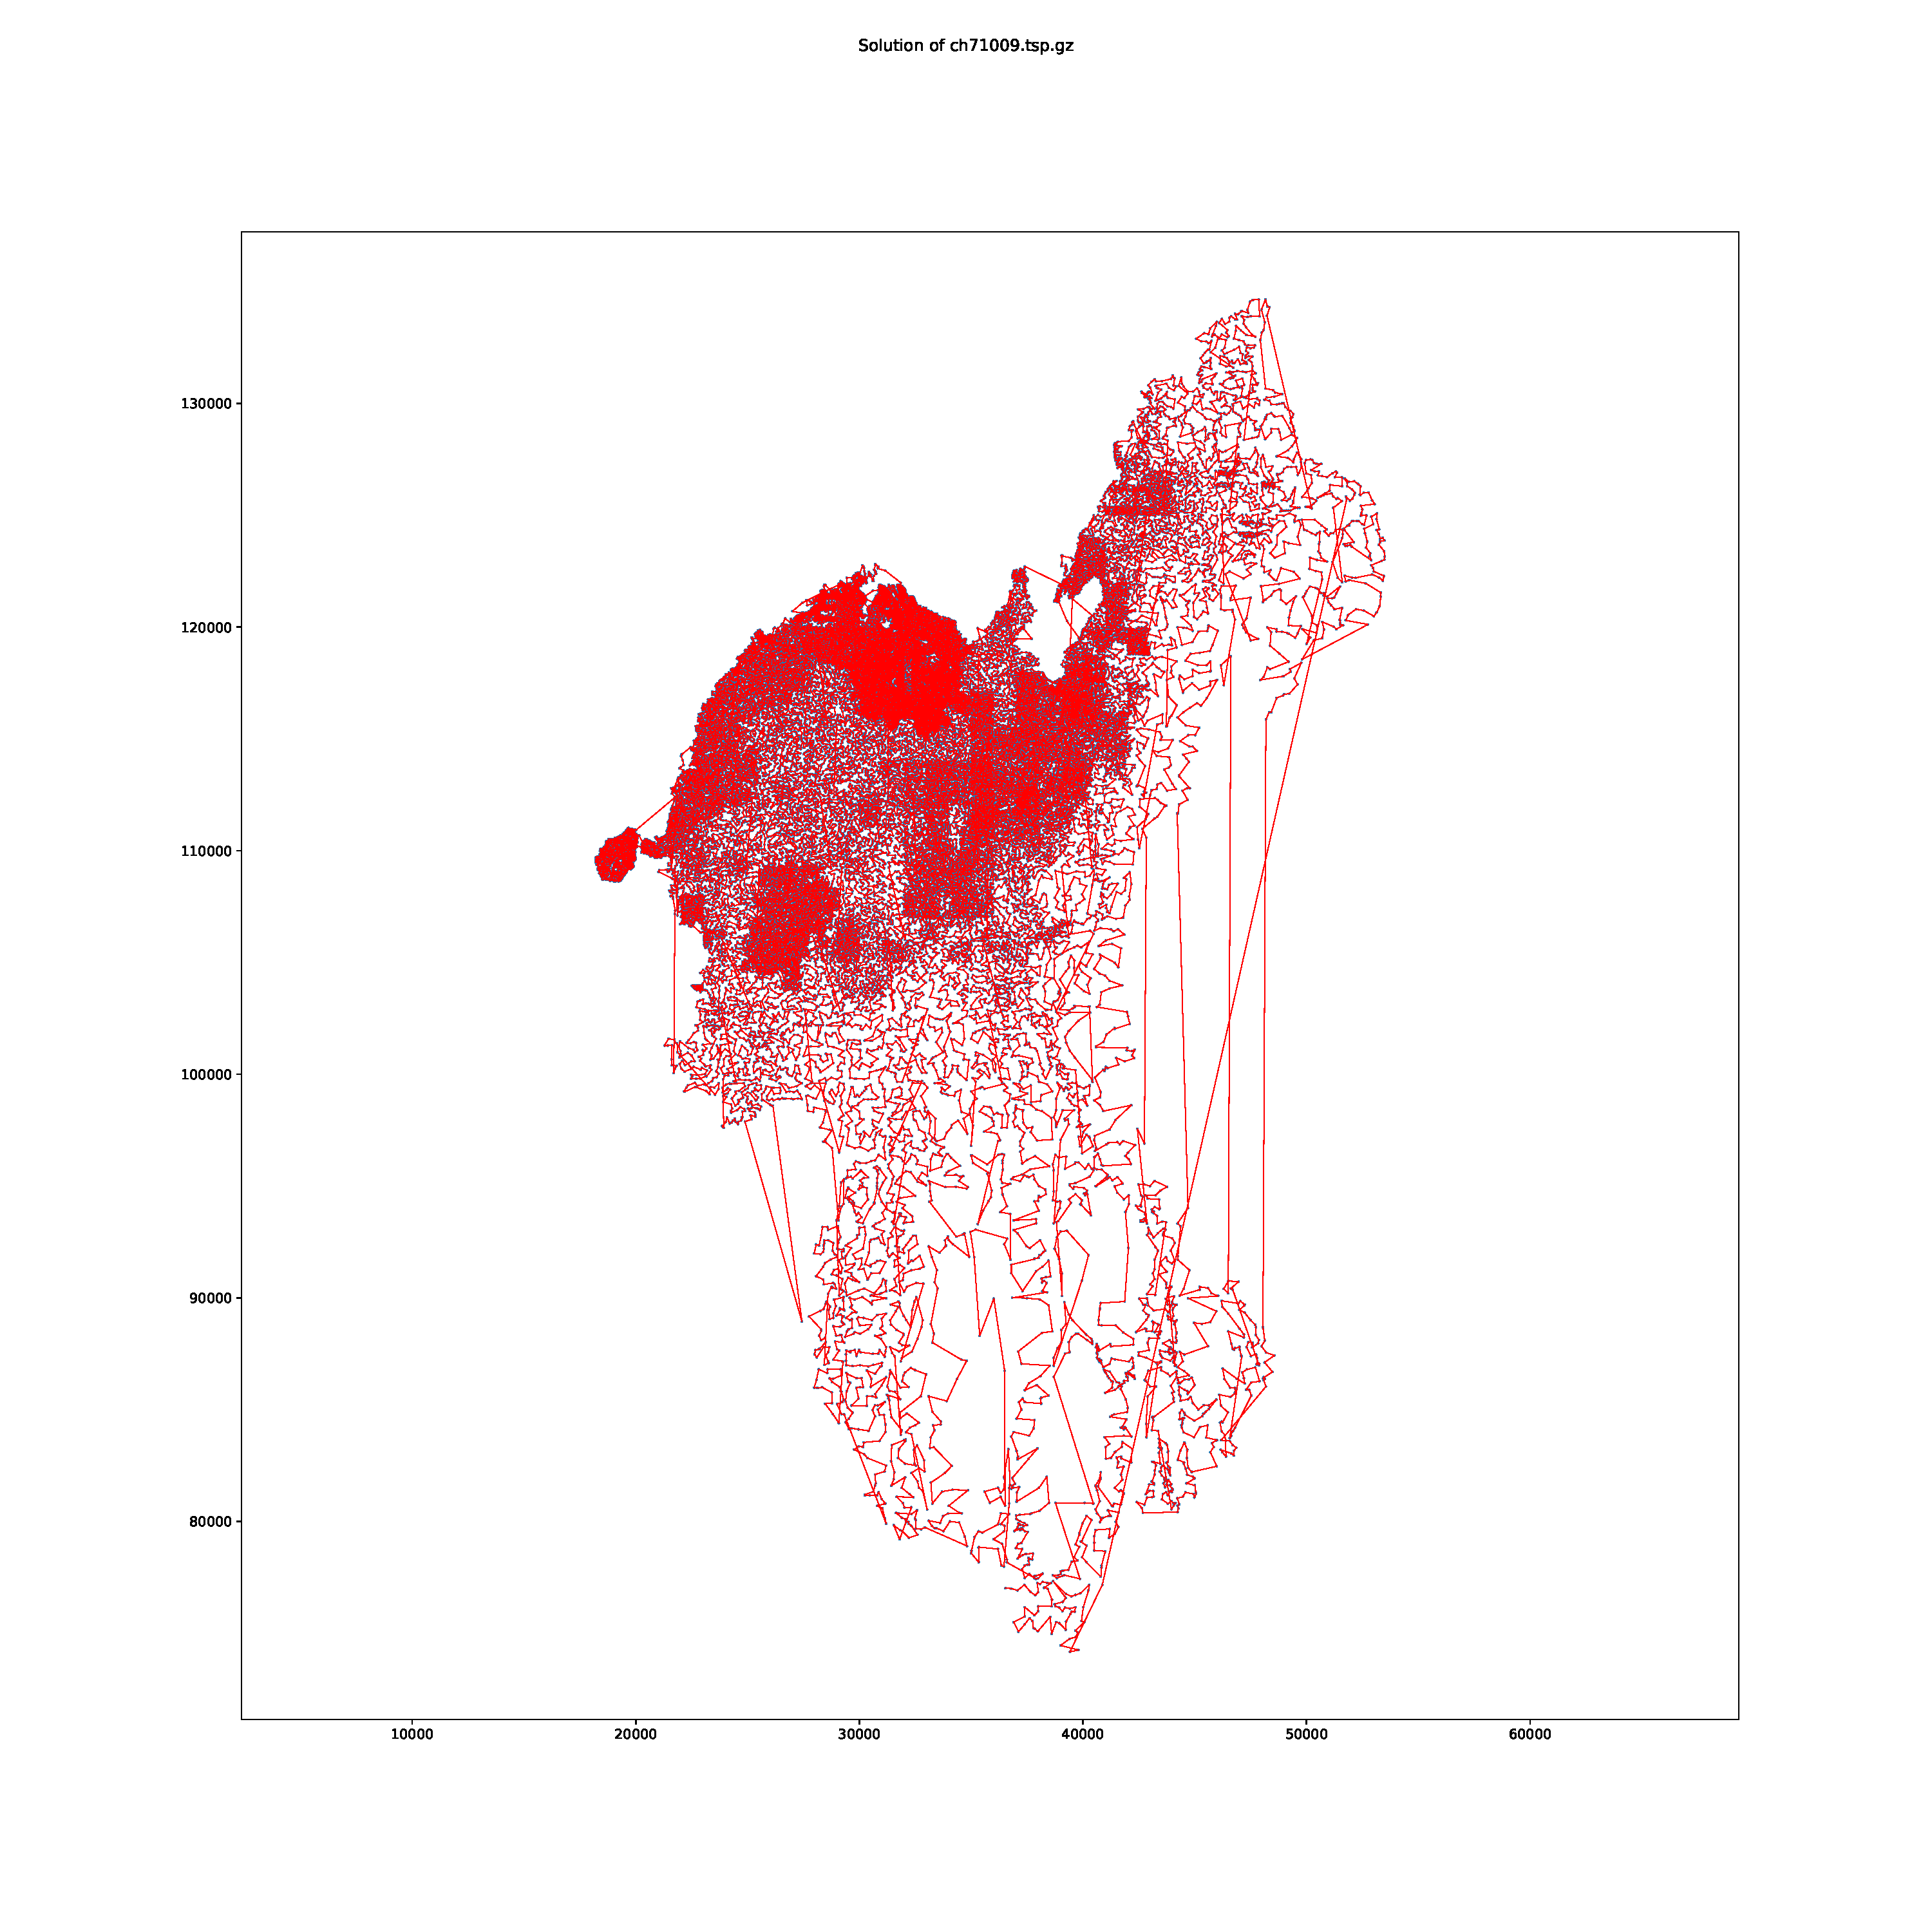
\includegraphics[width=\columnwidth, keepaspectratio]{grid_localopt_snake_ch71009.tsp.gz.pdf}

		\column{0.55\textwidth}
		Idea:
		\begin{itemize}
			\item Griddify graph
			\item stitch grid cells in snake order
			\item run 2opt on grid cells
		\end{itemize}
		
		But:
		\begin{itemize}
			\item locally nice..
			\item .. but merge step too bad
			\item bad solution quality
		\end{itemize}
	\end{columns}
\end{frame}


\begin{frame}{KD-Tree (limited depth)}
	\begin{columns}
		\column{0.4\textwidth}
		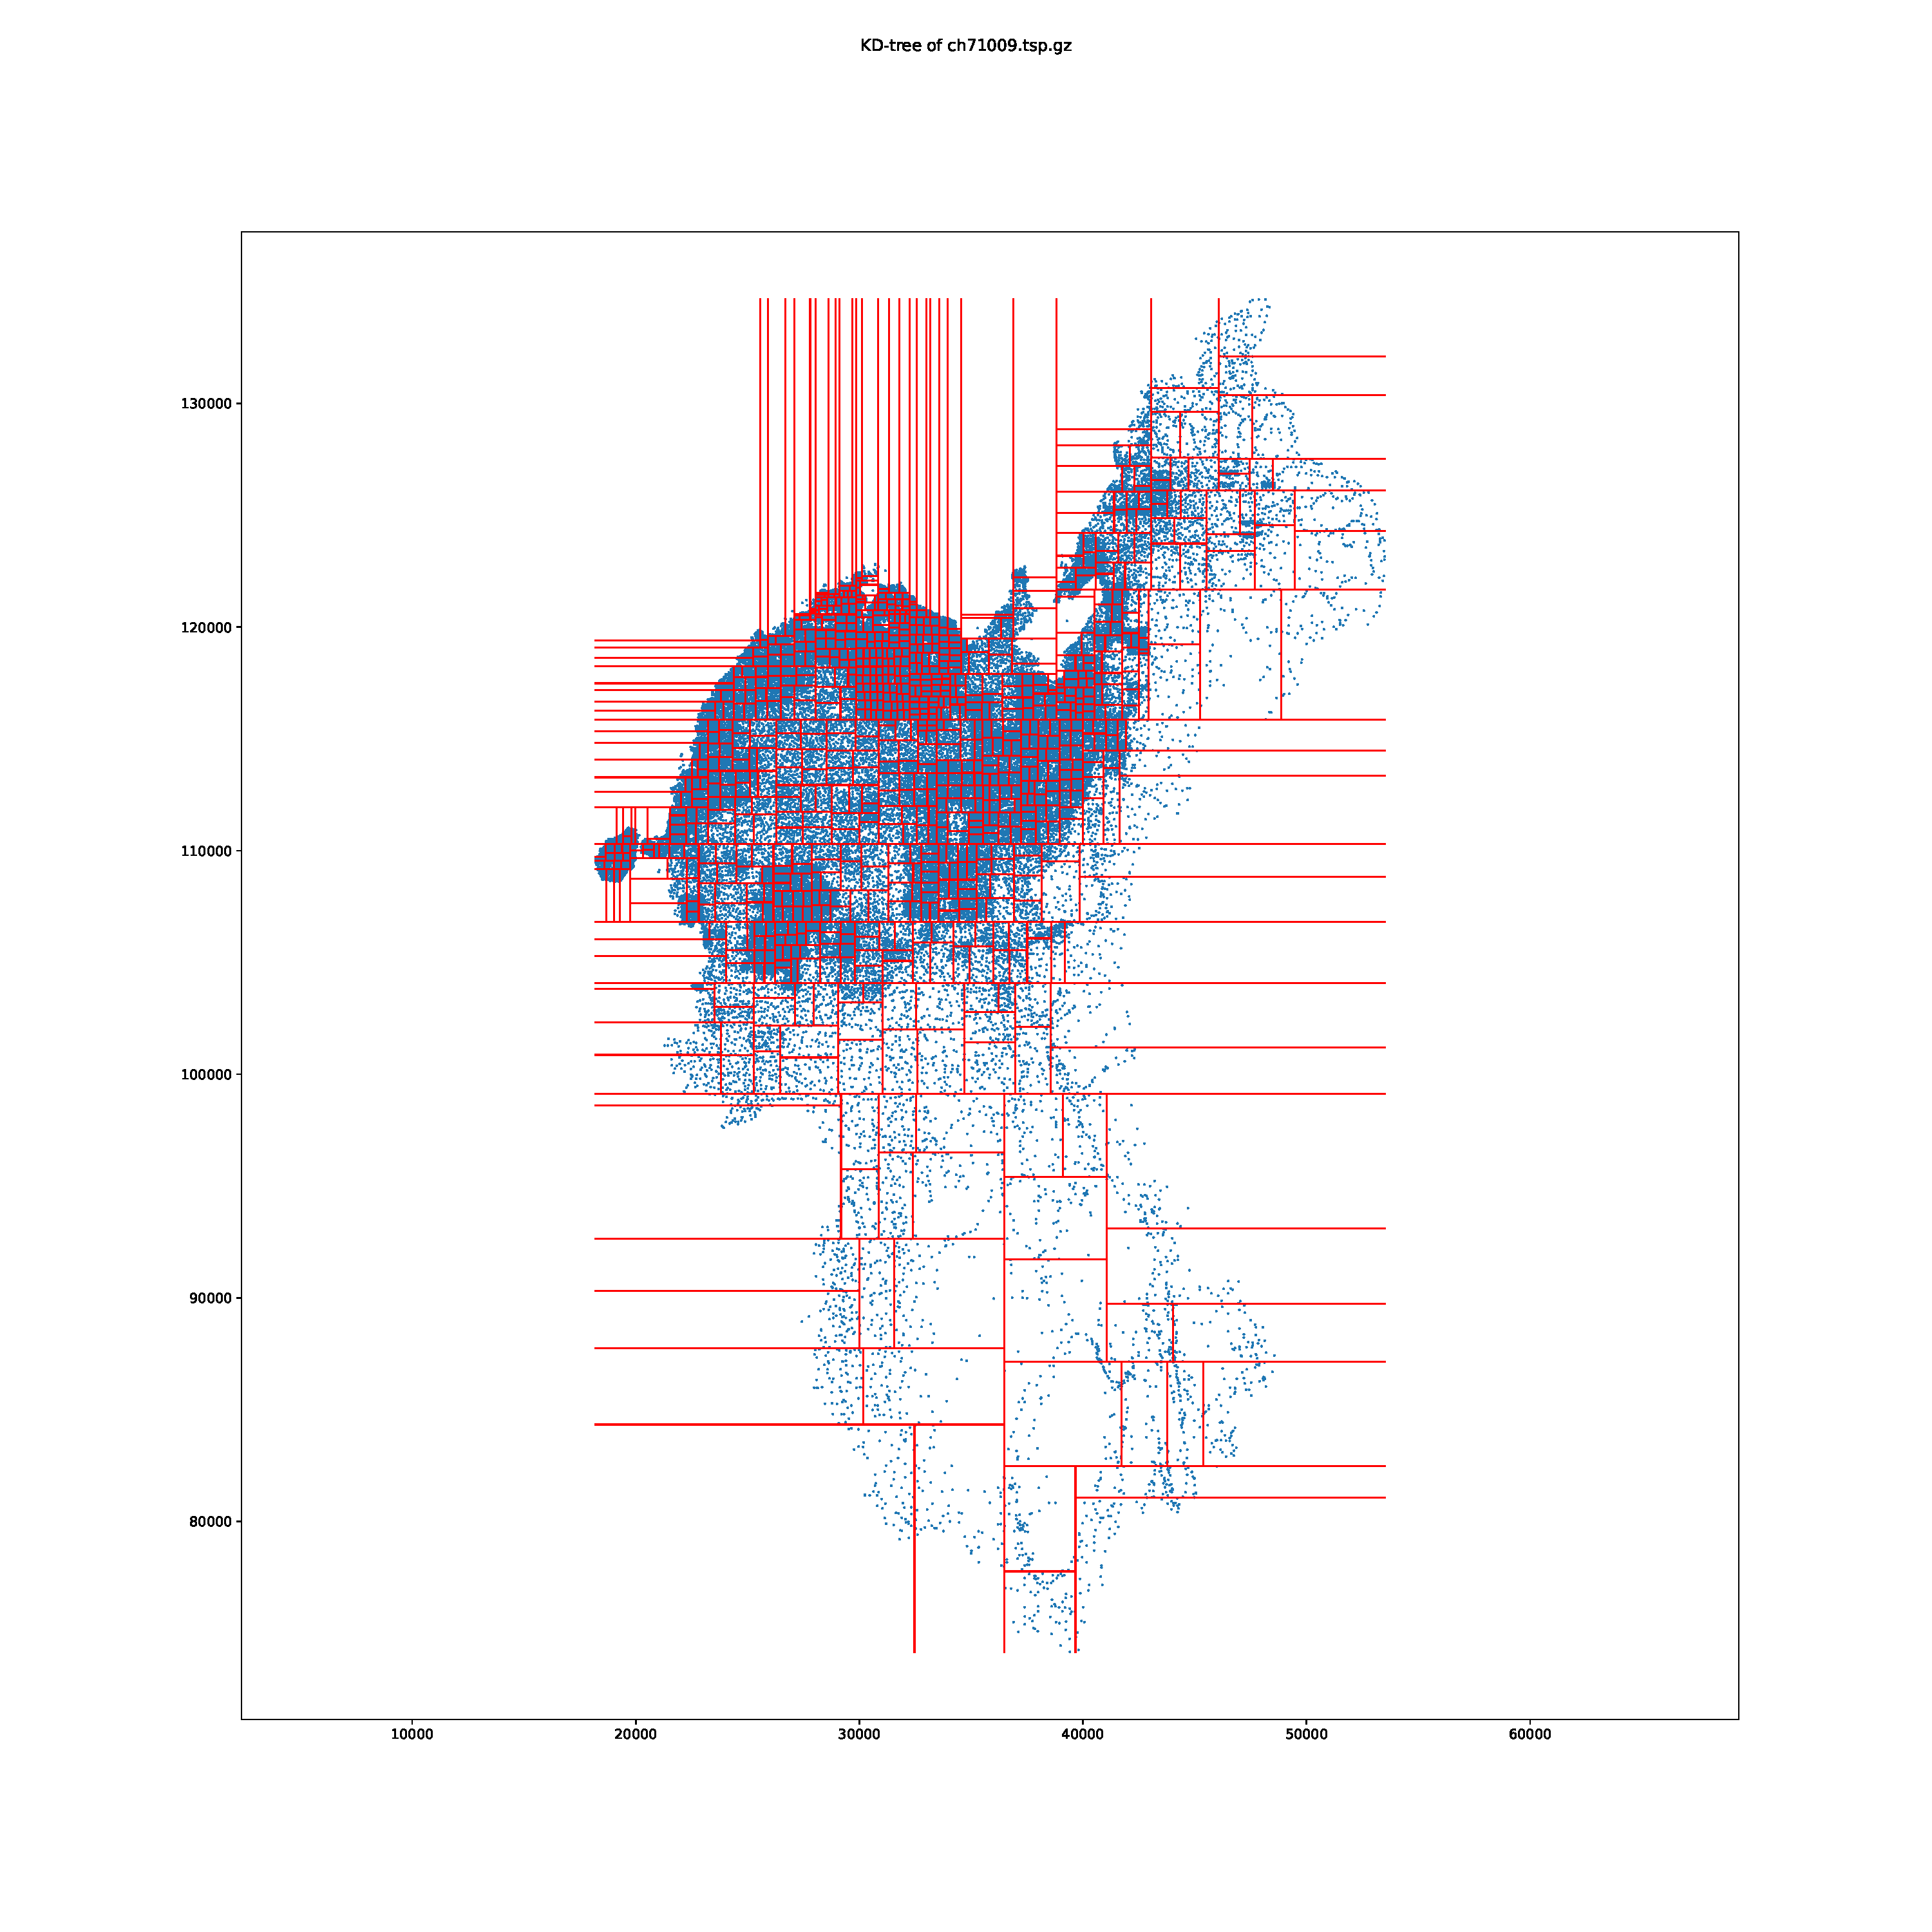
\includegraphics[width=\columnwidth, keepaspectratio]{kdtree_ch71009.tsp.gz.pdf}
		
		\column{0.55\textwidth}
		\begin{itemize}
			\item querys decide based on median
			\item very good balance
			\item but search requires a lot of memory accesses (median reads)
		\end{itemize}
	\end{columns}
\end{frame}


\begin{frame}{Quad-Tree}
	\begin{columns}
		\column{0.4\textwidth}
		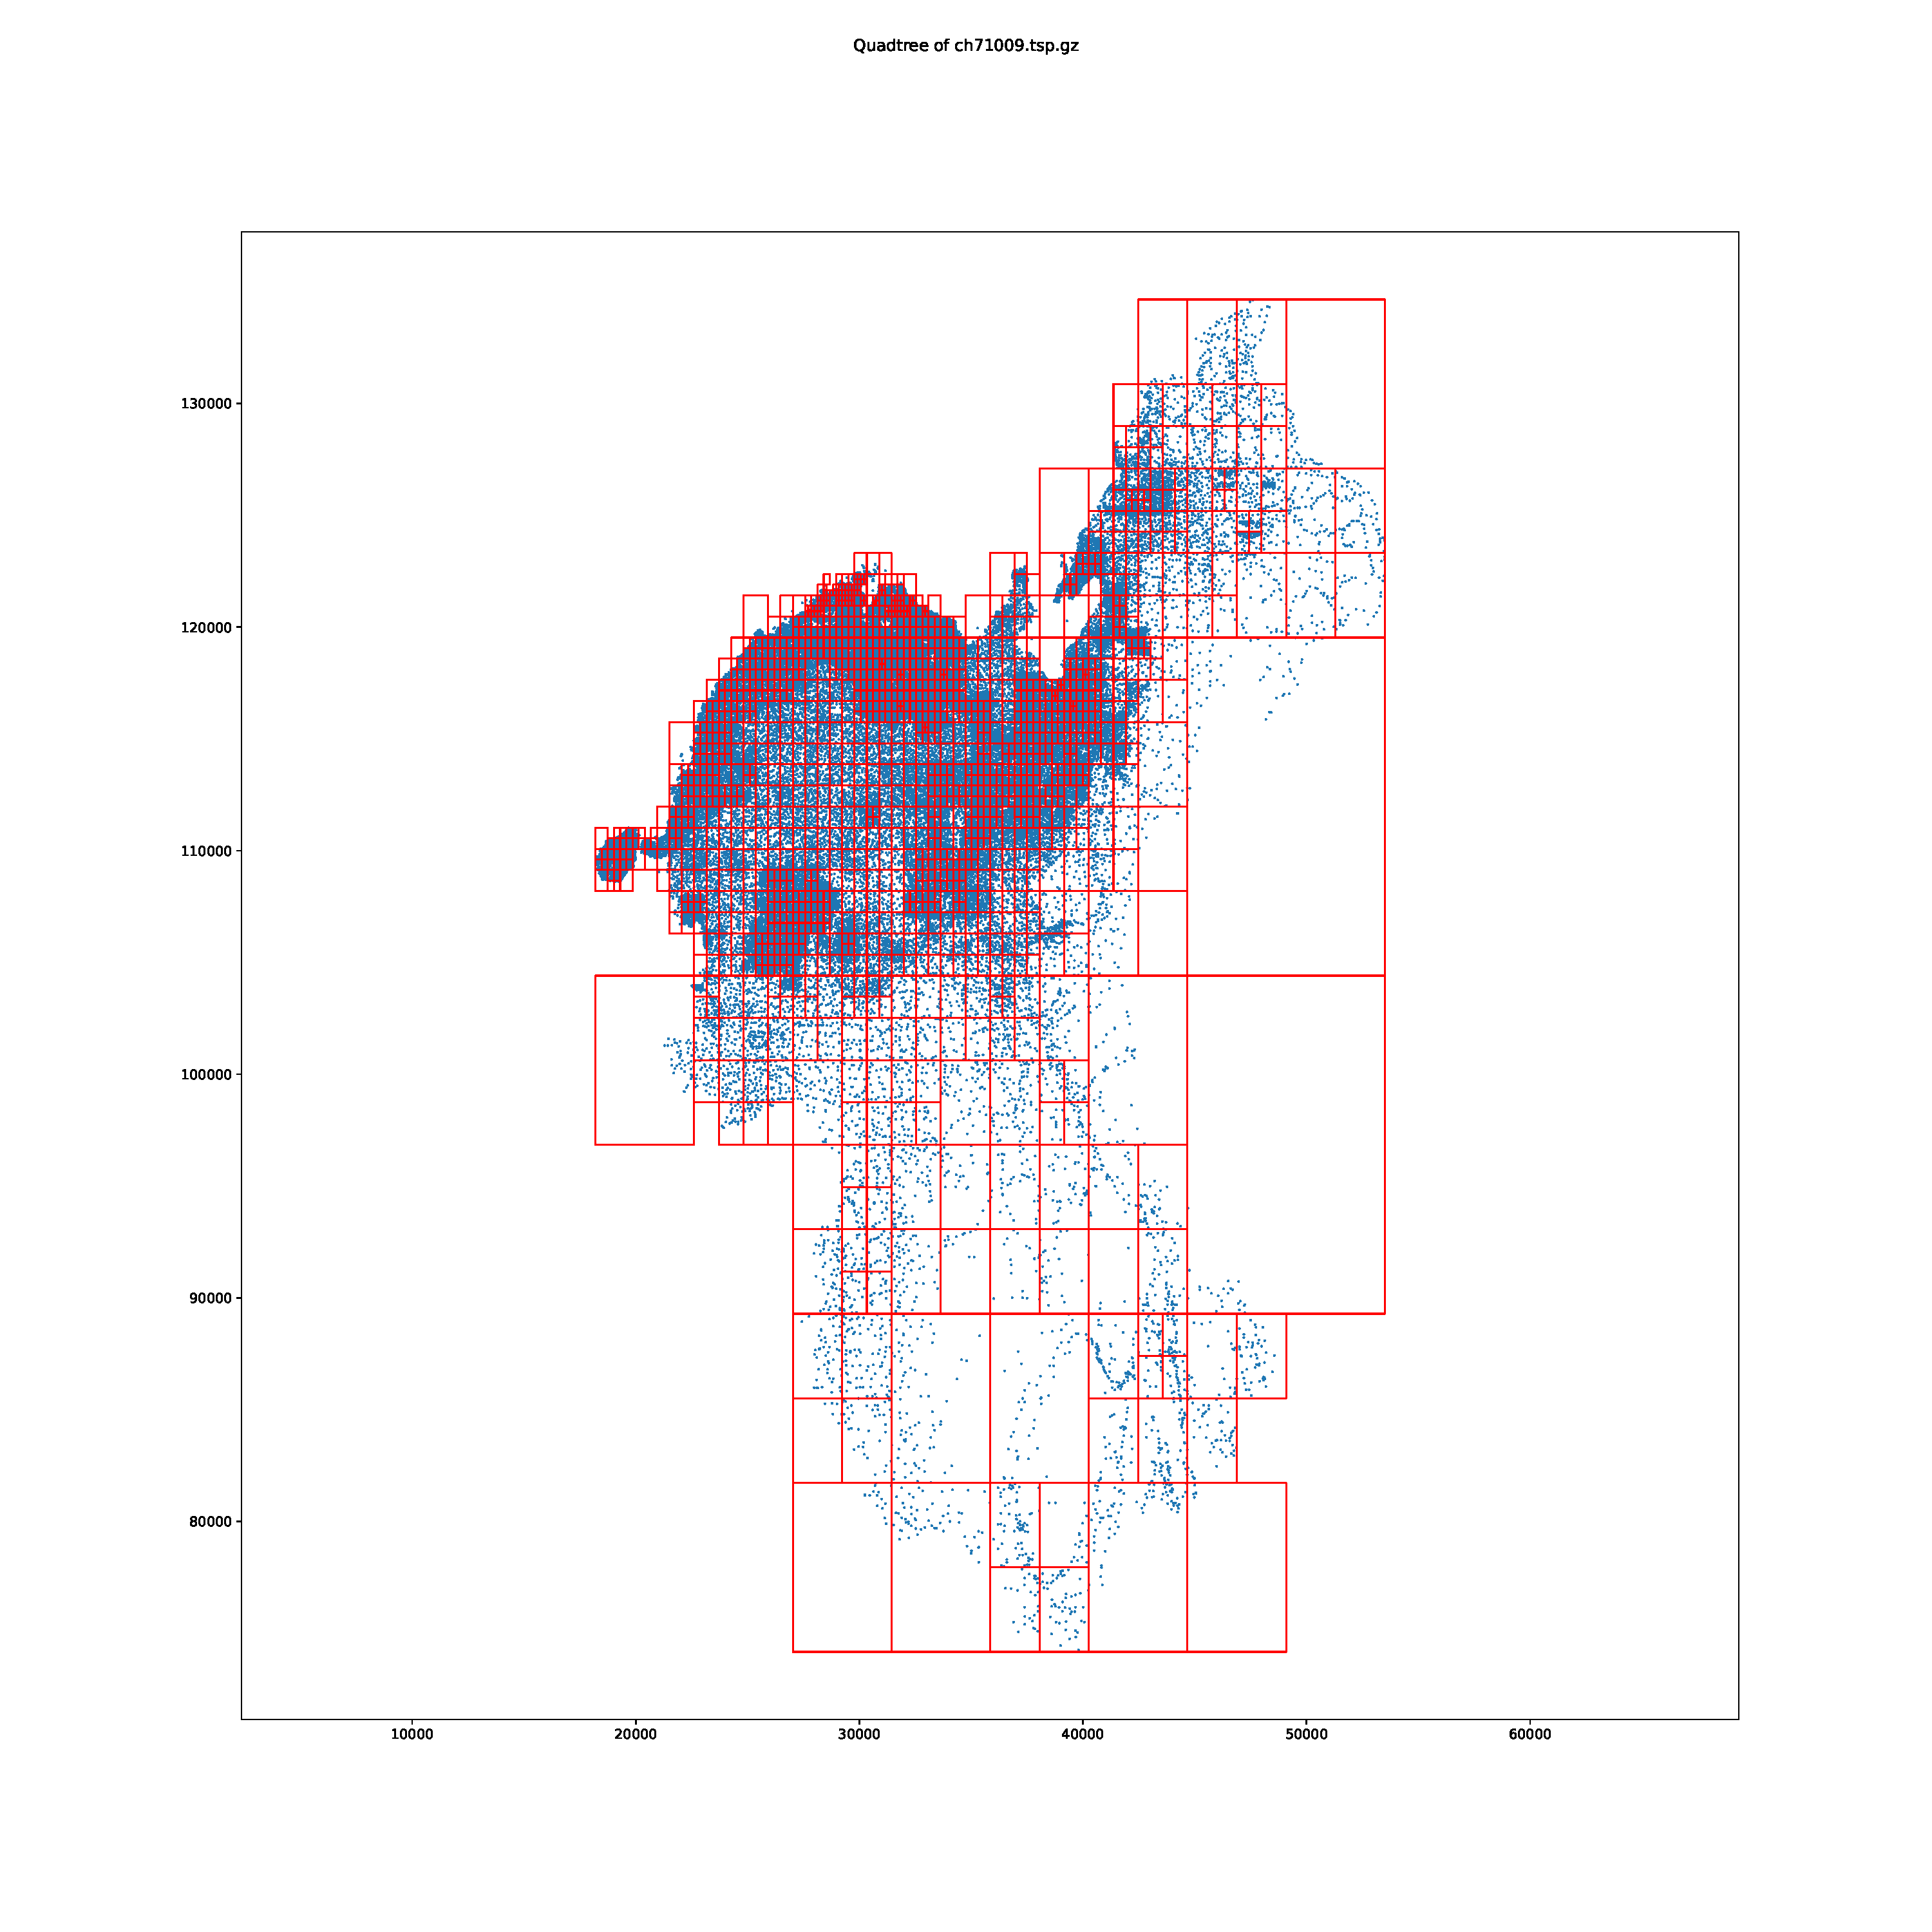
\includegraphics[width=\columnwidth, keepaspectratio]{quadtree_ch71009.tsp.gz.pdf}
		
		\column{0.55\textwidth}
		\begin{itemize}
			\item querys decide based on BBOX
			\item balance not ideal
			\item search can require very few memory reads: 
			\begin{itemize}
				\item branch not data-dependent
				\item implicit layout -> no pointers
				\item bitvector for node presence/status
			\end{itemize}
		\end{itemize}
	\end{columns}
\end{frame}

\begin{frame}{Greedy: Nearest Neighbour}
	\begin{columns}
		\column{0.4\textwidth}
		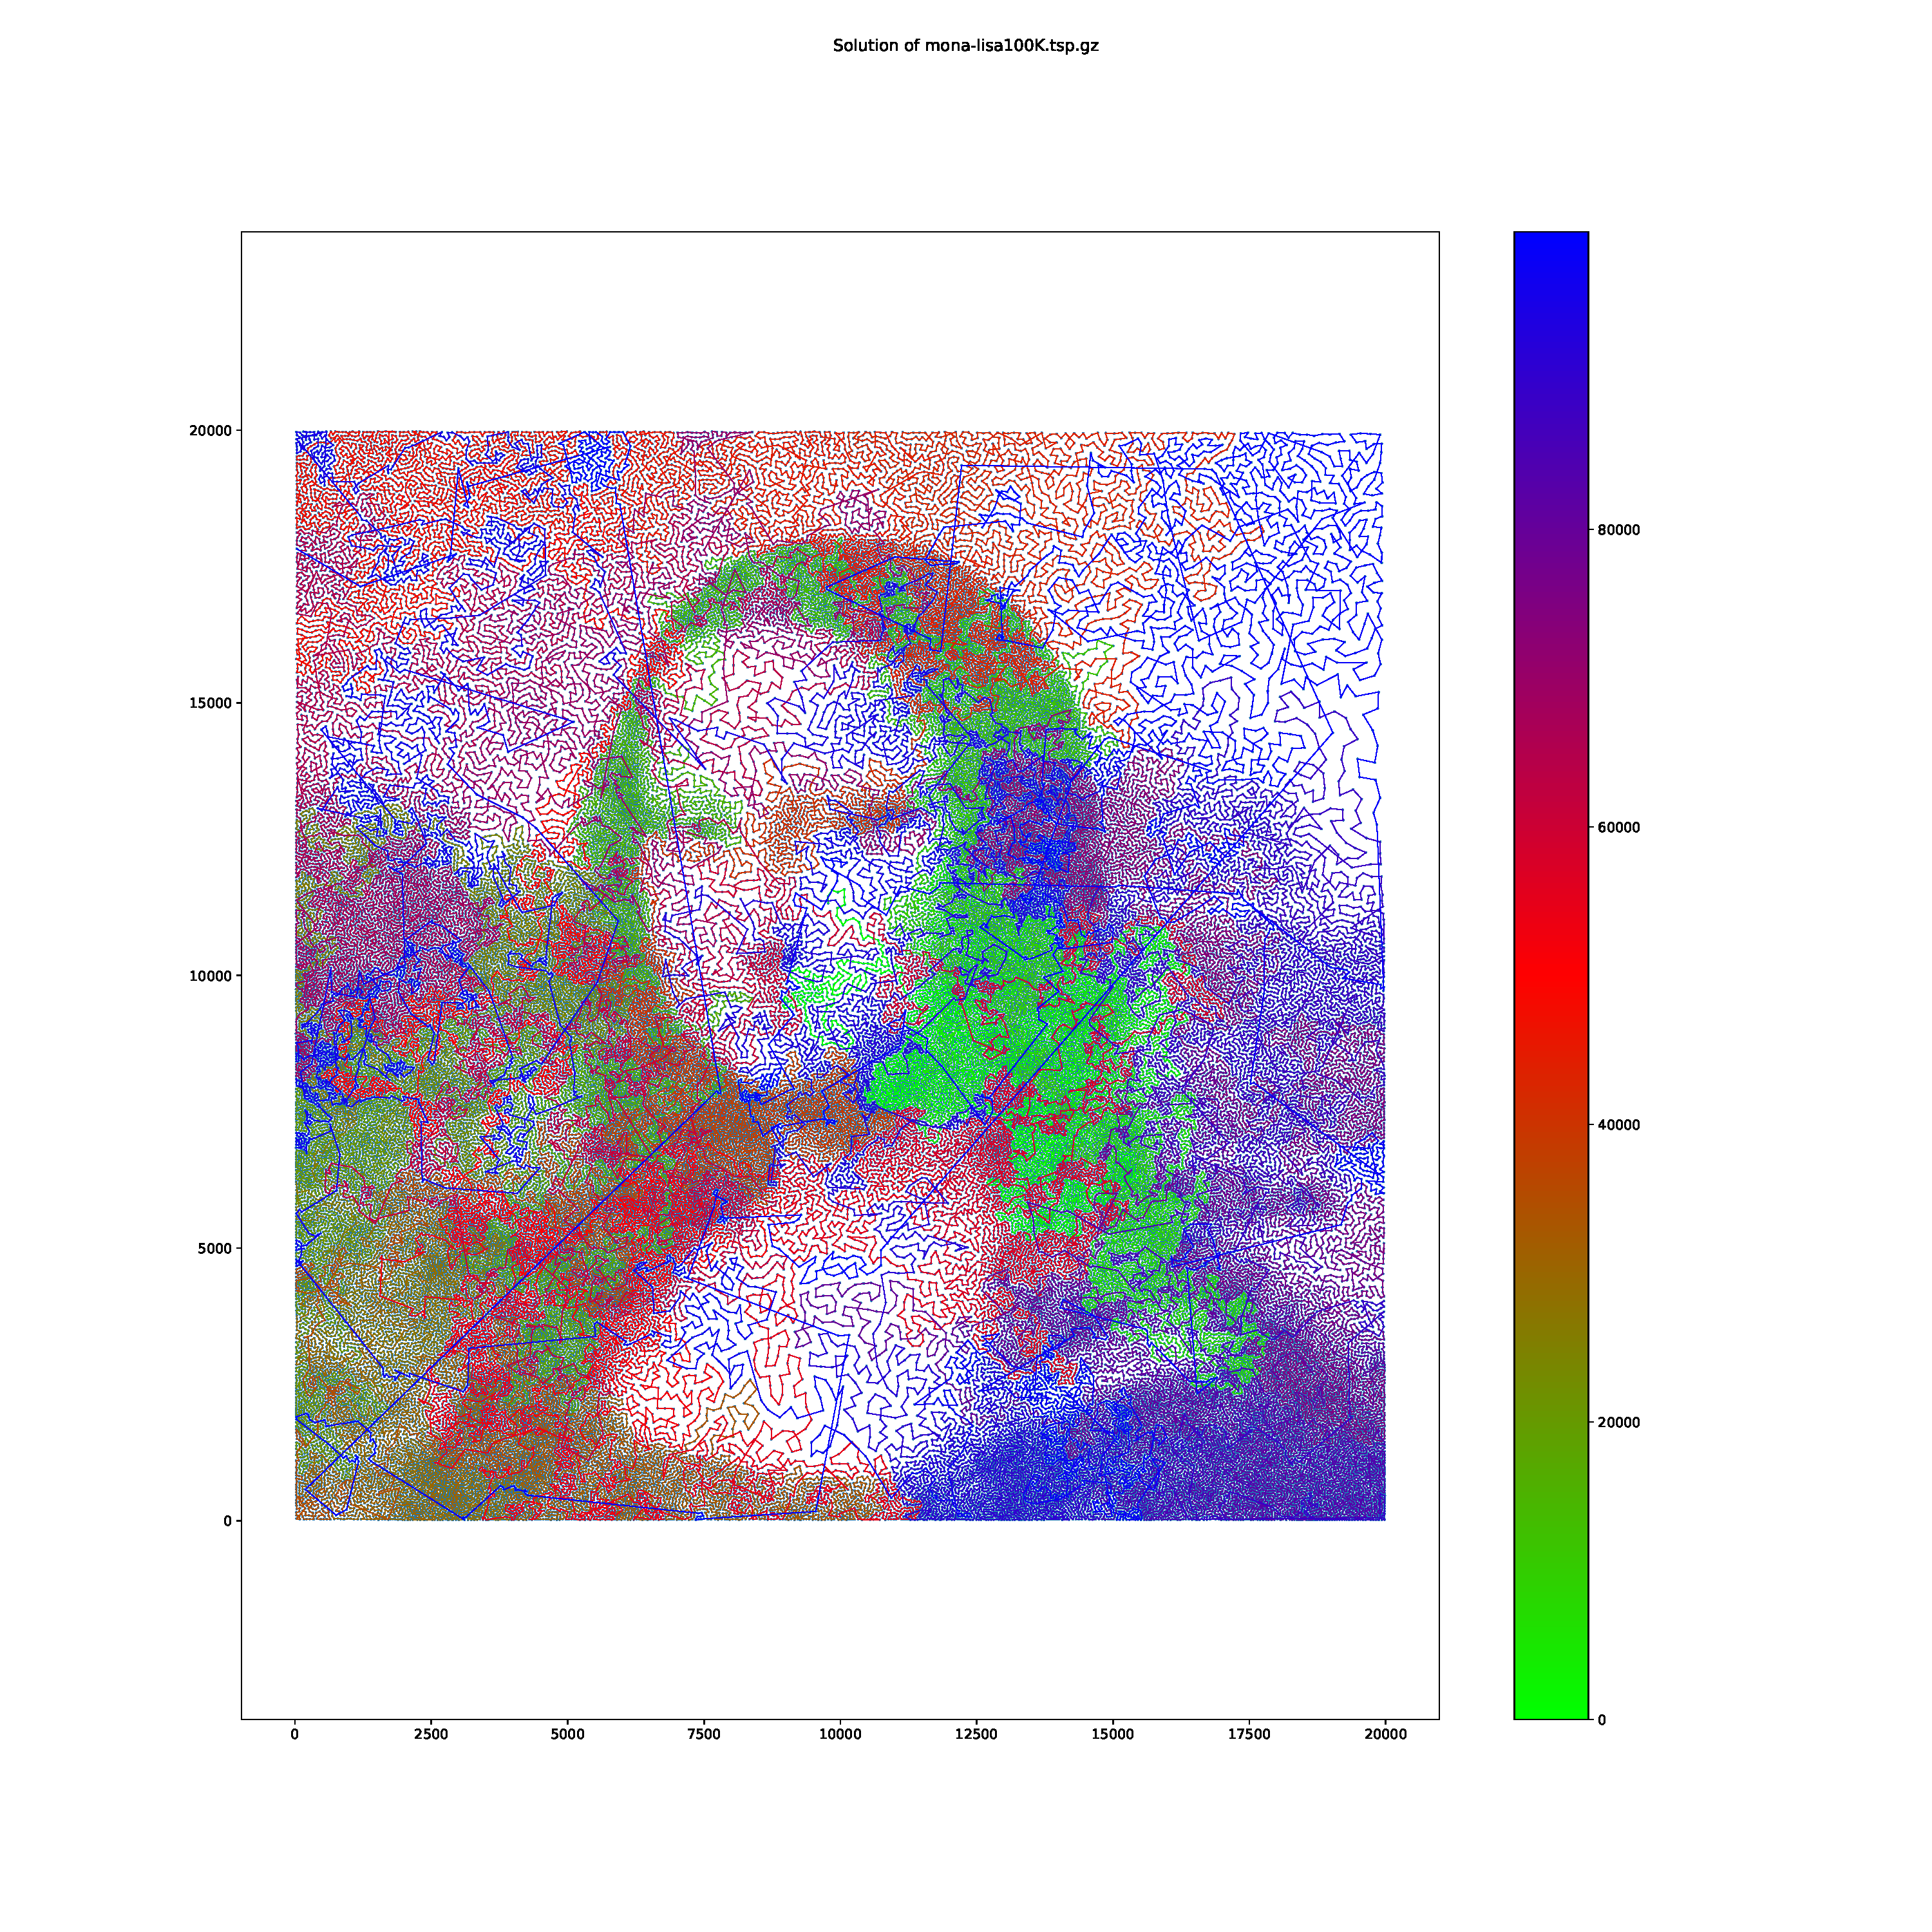
\includegraphics[width=\columnwidth, keepaspectratio]{nearest_neighbour_mona-lisa100K.tsp.gz.pdf}
		
		\column{0.55\textwidth}
		\begin{itemize}
			\item very fast
			\item solution quality much better
			\item but.. not quite good enough.
			\item especially later parts of the tour often cross
		\end{itemize}
	\end{columns}
\end{frame}

\begin{frame}{Greedy: Nearest Neighbour (multishot)}
	\begin{columns}
		\column{0.4\textwidth}
		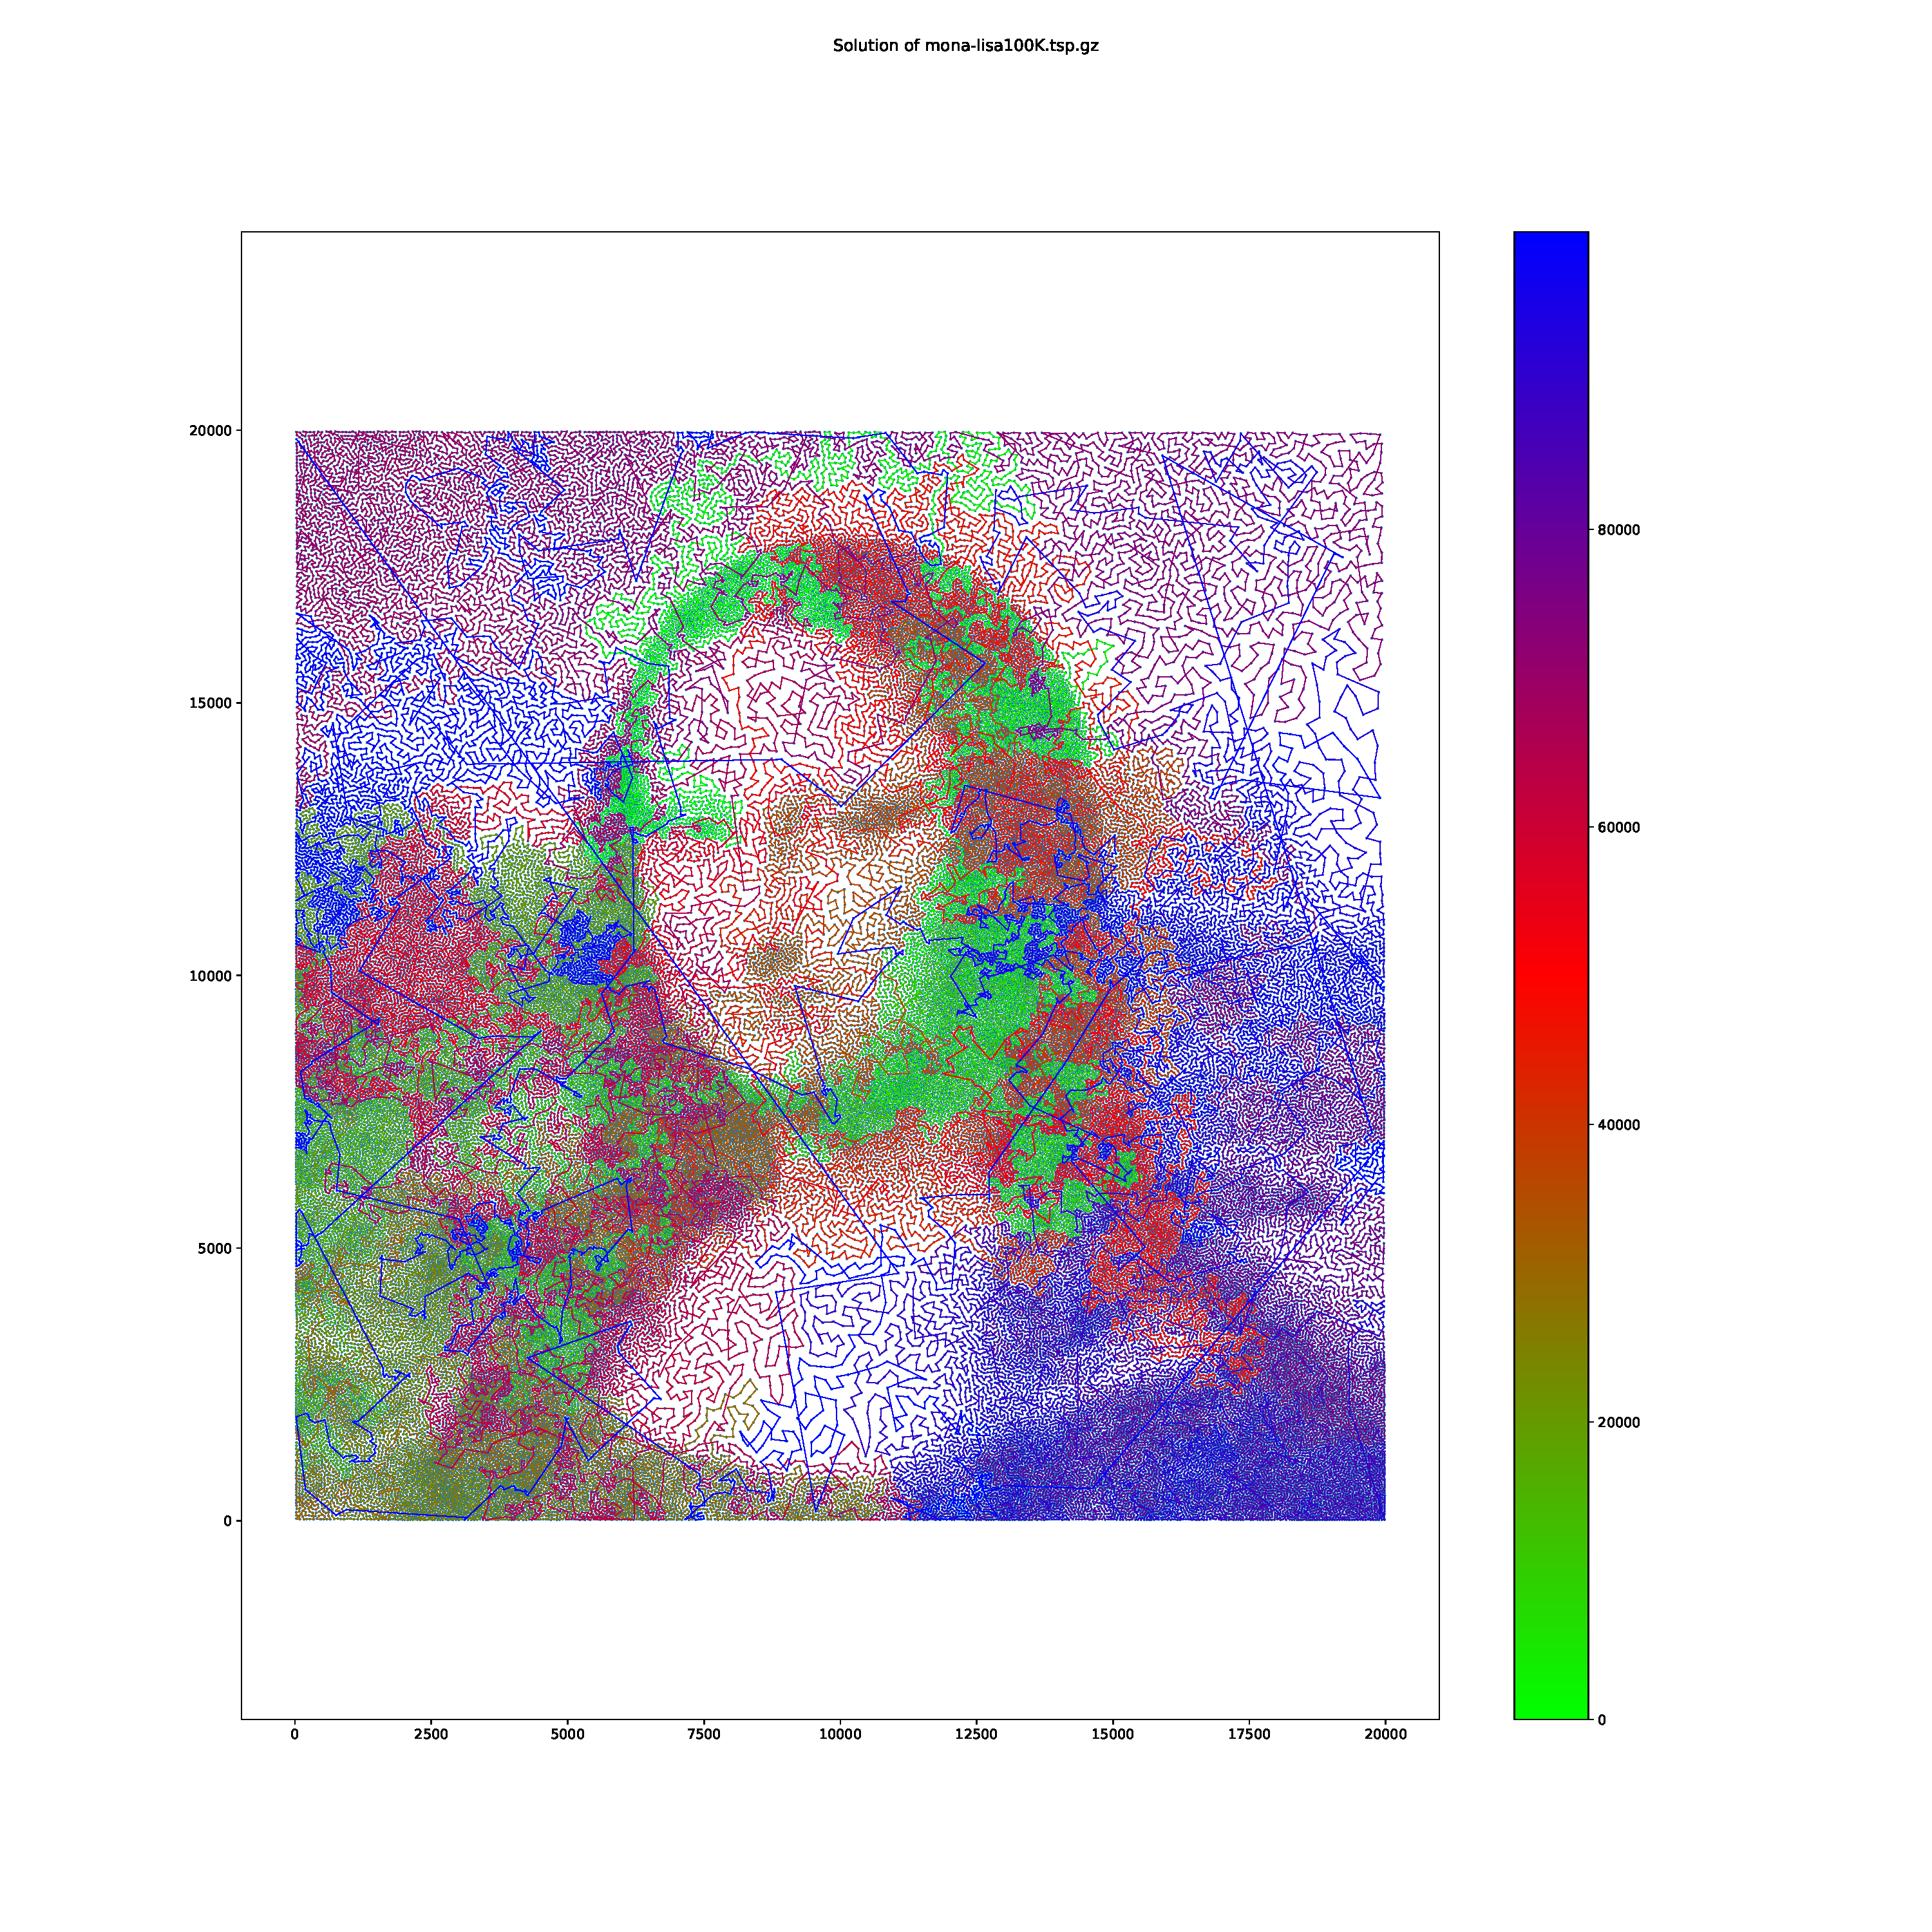
\includegraphics[width=\columnwidth, keepaspectratio]{nearest_neighbour_multishot_mona-lisa100K.tsp.gz.pdf}
		
		\column{0.55\textwidth}
		multiple attempts, similar to Sheet 1 Ex 03c
		
		\begin{tblr}{colspec={c|r|r|r}}
			instance & tourlen & time & gap \\
			sw24978 & 1,057,479 & \qty{0.05}{\second} & \qty{23.6}{\percent} \\
			ch71009 & 5,629,180 & \qty{0.14}{\second} & \qty{23.3}{\percent} \\
			mona-lisa100K & 6,868,893 & \qty{0.22}{\second} & \qty{19.3}{\percent} \\
			lra498378 & 2,690,495 & \qty{1.00}{\second} & \qty{24.1}{\percent} \\
		\end{tblr}

		PASSED
	\end{columns}
\end{frame}

\begin{frame}{Greedy: Nearest Neighbour + twoopt}
	\begin{columns}
		\column{0.4\textwidth}
		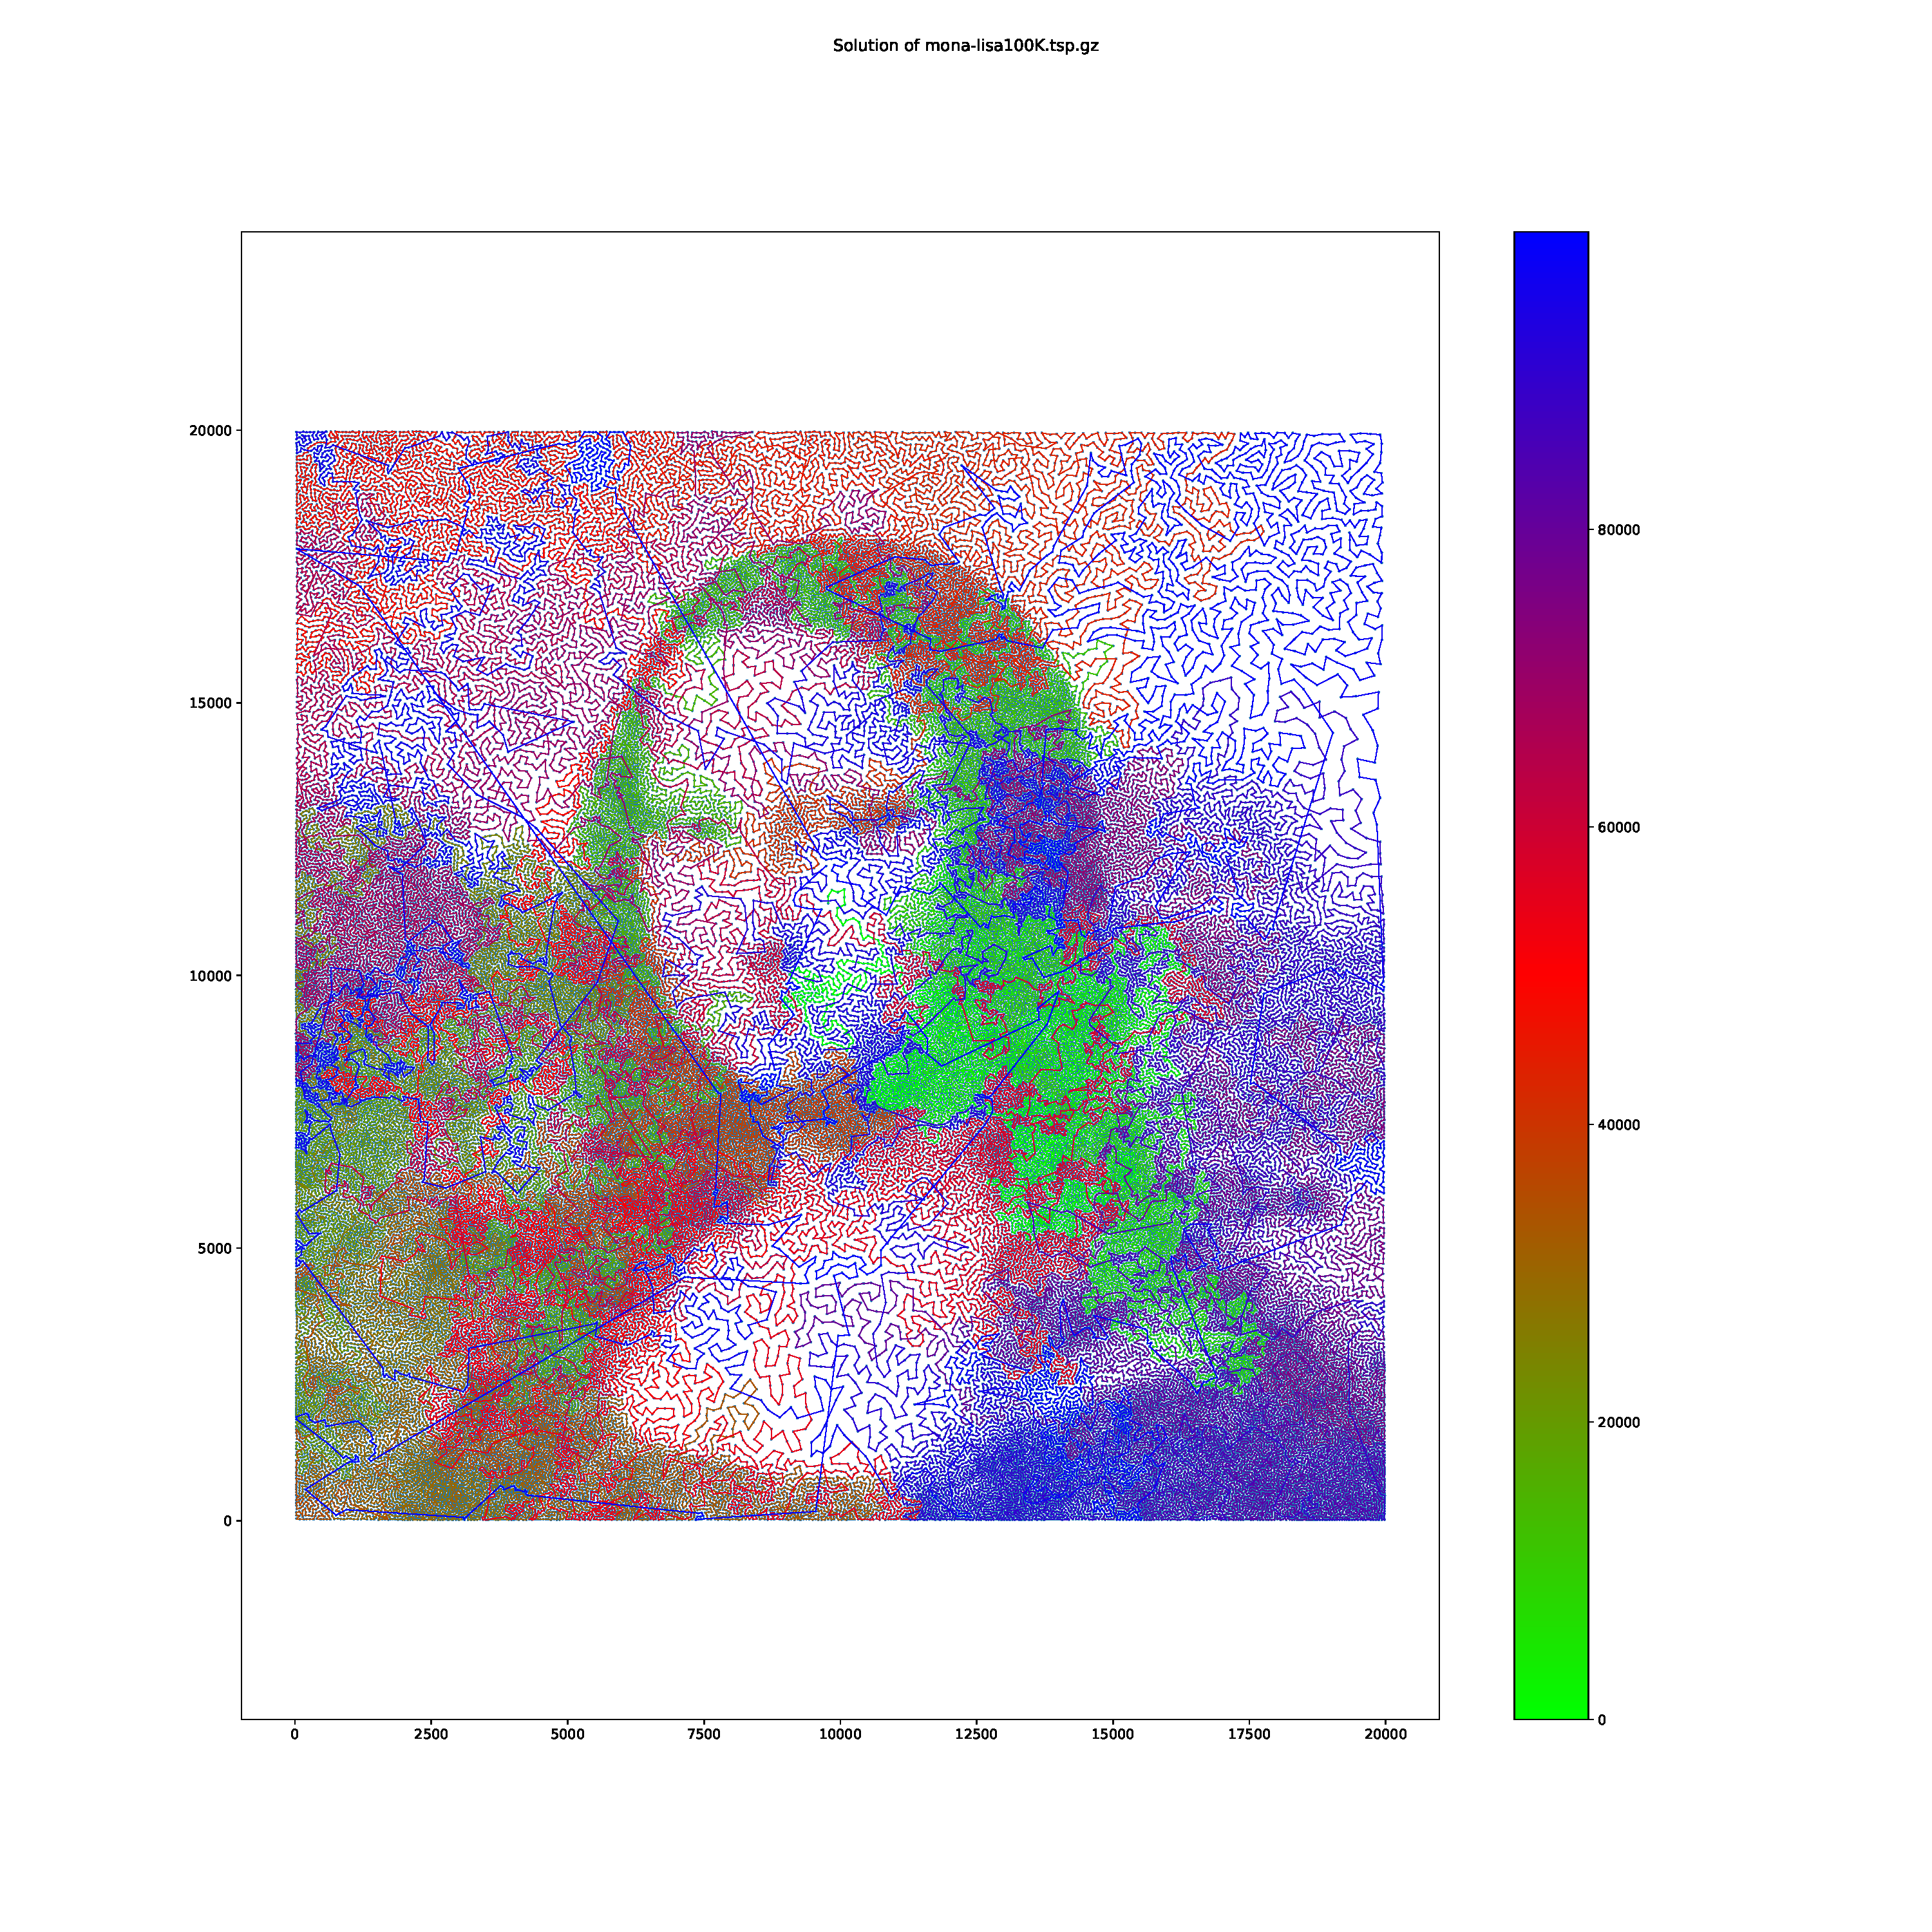
\includegraphics[width=\columnwidth, keepaspectratio]{nearest_neighbour_twoopt_mona-lisa100K.tsp.gz.pdf}
		
		\column{0.55\textwidth}
		add twoopt-passes
		\begin{itemize}
			\item windowed 2opt (200 interval) $\implies \mathcal{O}(n)$
			\item section twoopt (last 2000) $\implies \mathcal{O}(1)$
		\end{itemize}
		
		\begin{tblr}{colspec={c|r|r|r}}
			instance & tourlen & time & gap \\
			sw24978 & 994,382 & \qty{0.27}{\second} & \qty{16.2}{\percent} \\
			ch71009 & 5,355,160 & \qty{0.52}{\second} & \qty{17.3}{\percent} \\
			mona-lisa100K & 6,554,454 & \qty{0.66}{\second} & \qty{13.8}{\percent} \\
			lra498378 & 2,563,243 & \qty{3.92}{\second} & \qty{18.2}{\percent} \\
		\end{tblr}
		
		PASSED
	\end{columns}
\end{frame}

\begin{frame}{Other Heuristics...}
	\href{https://hal.science/hal-04909391v2/file/TSP_2024_V1.11.pdf}{https://hal.science/hal-04909391v2/file/TSP\_2024\_V1.11.pdf}
	\begin{columns}[T]
		\column{0.45\textwidth}
		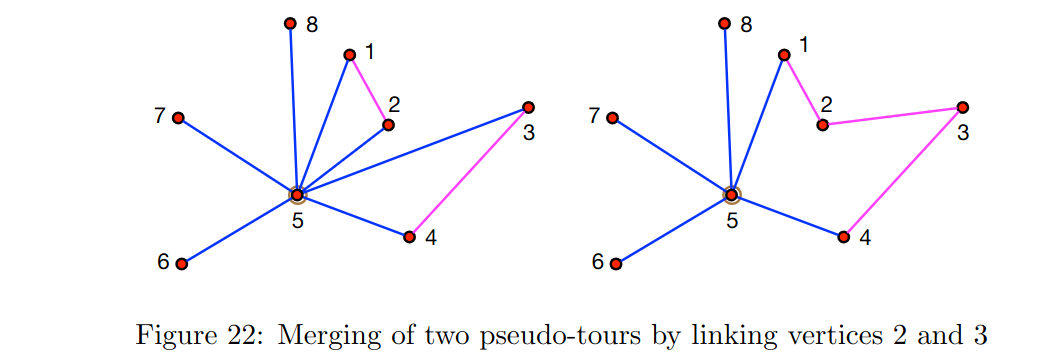
\includegraphics[width=\columnwidth, keepaspectratio]{clarke_wright.png}
		\column{0.45\textwidth}
		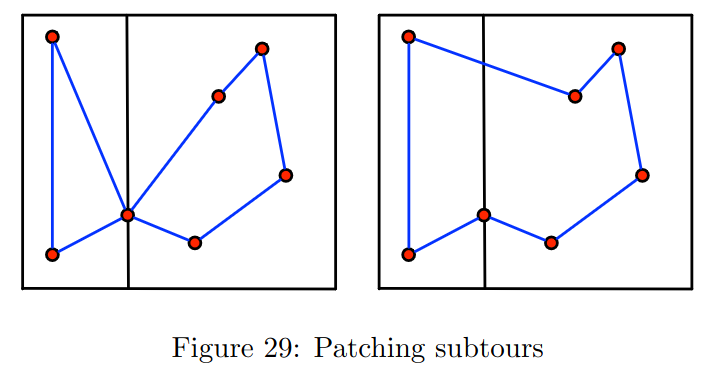
\includegraphics[width=\columnwidth, keepaspectratio]{patching.png}
	\end{columns}
\end{frame}

\begin{frame}{Other Heuristics...}
	\href{https://hal.science/hal-04909391v2/file/TSP_2024_V1.11.pdf}{https://hal.science/hal-04909391v2/file/TSP\_2024\_V1.11.pdf}
	\begin{columns}[T]
		\column{0.45\textwidth}
		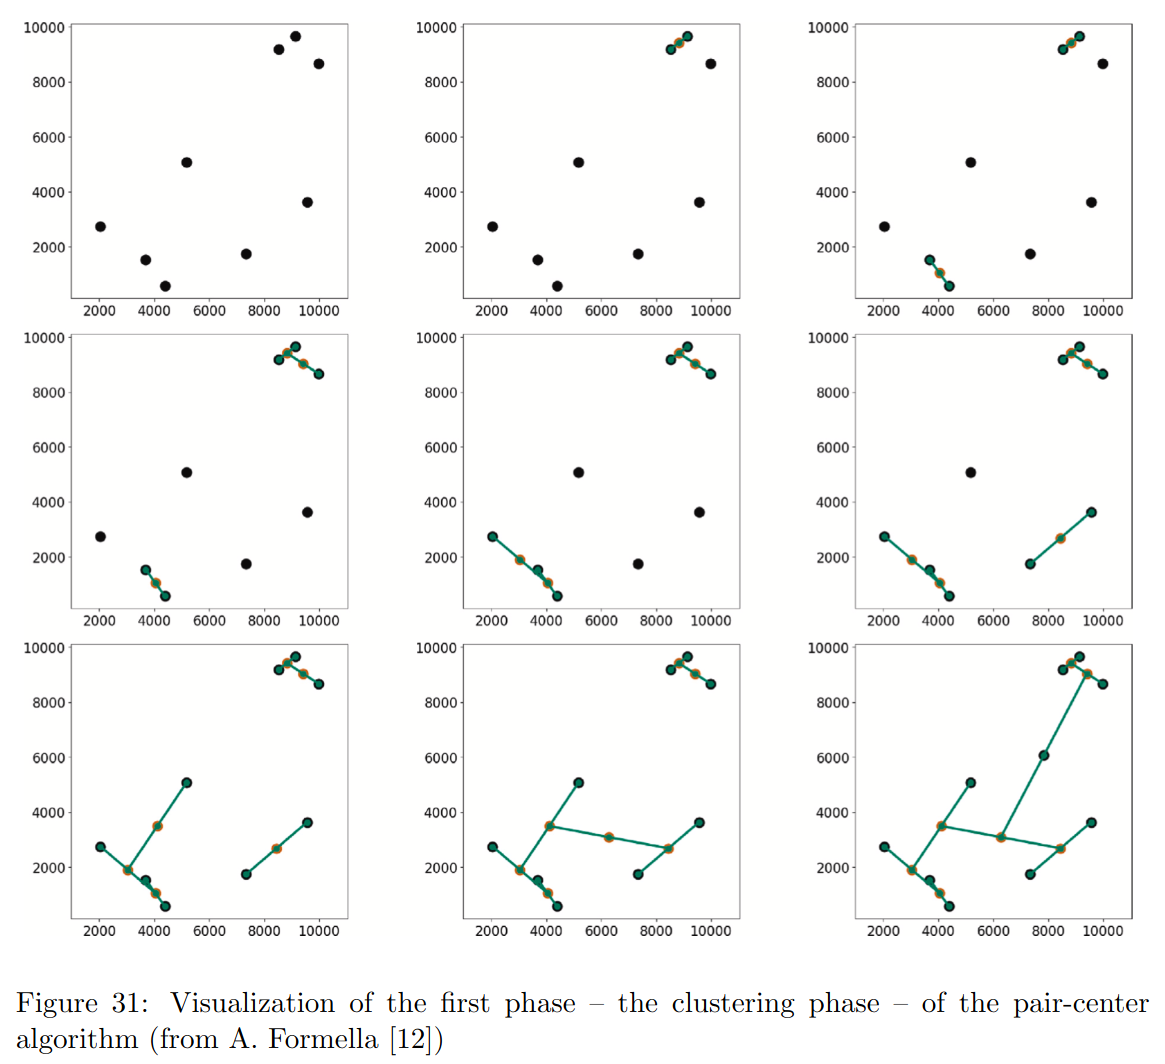
\includegraphics[width=\columnwidth, keepaspectratio]{pair_center_1.png}
		\column{0.45\textwidth}
		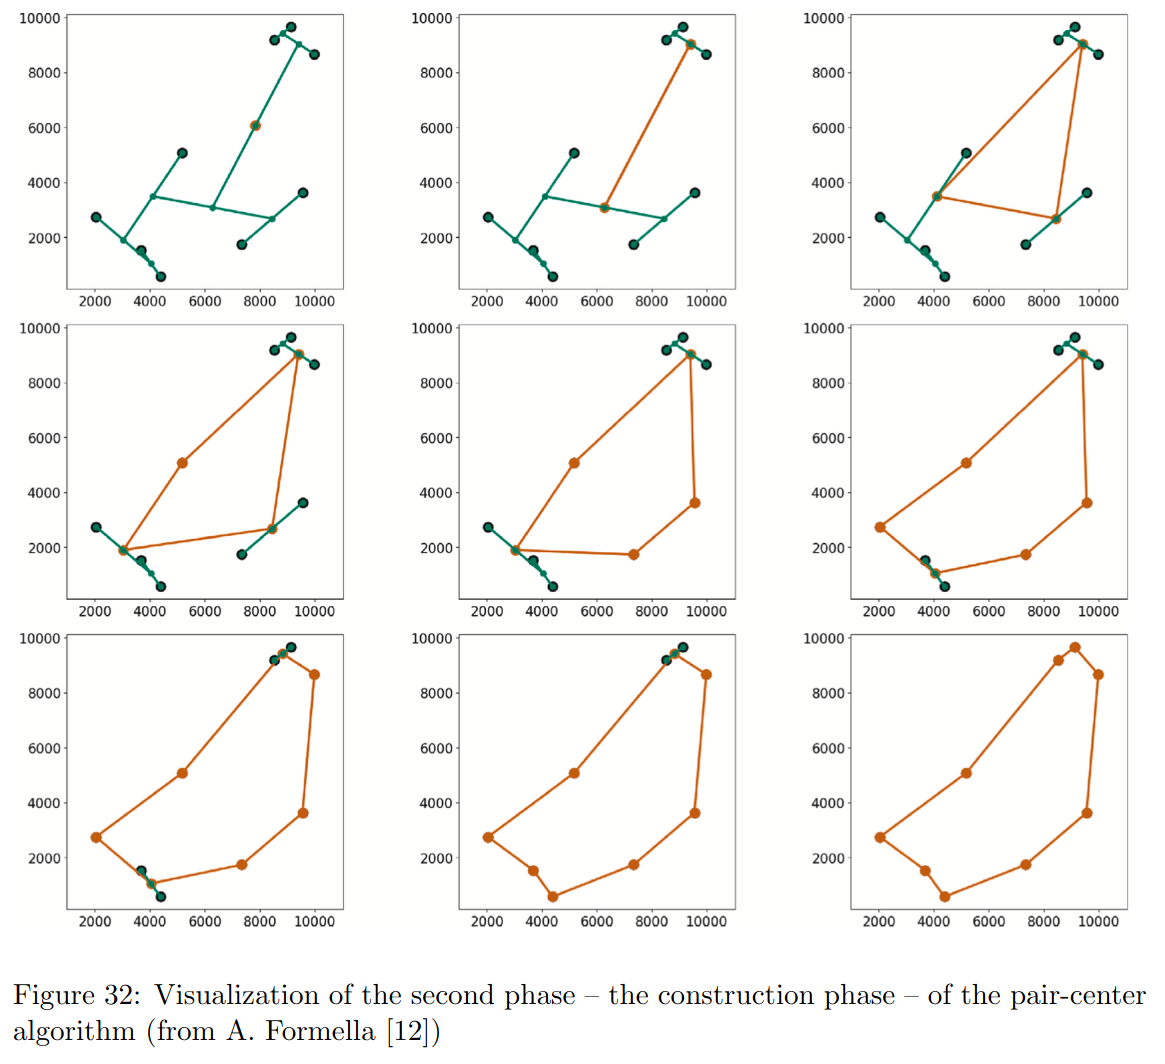
\includegraphics[width=\columnwidth, keepaspectratio]{pair_center_2.png}
	\end{columns}
\end{frame}

\end{document}


